\section{Survey methodology}
\label{sec:method}

\subsection{Search, deduplication and placement}
\label{sec:search}

The corpus was built from \nStreams web searches run on \searchDate, one per slice of the pipeline: the
model's read-off and post-hoc maps (S0 and S1), prompt elicitation (S2), sampling-based and conformal
methods (two slices of S3), training (S4), the works that act on a confidence or fix the output
contract (X), and independent evaluations of Jev, a hosted typed-decision model released during the
search period. The query strings and the number of records screened
were not recorded; Figure~\ref{fig:prisma} marks those stages as not recorded rather than estimating
them. Records were matched on arXiv identifier, DOI and normalised title: \nDup duplicates were removed
and \nMapped records were matched to references already cited and kept, leaving \nWorks works.

% AUTO-GENERATED by build/gen_corpus.py -- counts from literature/merge_report.md, prior_surveys.md and the model snapshots; unrecorded counts are marked, never estimated.
\begin{figure}[t]
\centering
\begin{tikzpicture}[font=\footnotesize, box/.style={draw=black!55,rounded corners=3pt,align=center,text width=66mm,inner sep=4pt,fill=white},
  nl/.style={box,dashed,draw=black!40,text=black!55,fill=black!2}, side/.style={box,text width=53mm,fill=black!3},
  every node/.append style={execute at begin node={\hyphenpenalty=10000\exhyphenpenalty=10000}},
  ar/.style={-{Stealth[length=2.2mm]},black!60,line width=0.7pt}]
 \node[box] (id) {\textbf{Identification}: 7 web searches run on 2026-09-26 (queries not recorded)\\[2pt]
   records identified: S0 and S1 69, S2 67, S3 sampling 66, S3 conformal 64, S4 training 86, X consumers 77, independent evaluations of Jev 1; total 430};
 \node[nl, below=5mm of id]  (scr) {\textbf{Screening}: records screened and excluded \emph{not recorded}; each search kept only records whose title, first author, year and identifier were confirmed};
 \node[box, below=5mm of scr] (dup) {\textbf{Duplicates} (arXiv id, DOI, normalised title) removed: 22\\ records matched to references already cited (kept): 11};
 \node[box, below=5mm of dup] (inc) {\textbf{Included}: 408 works};
 \node[box, text width=31mm, below left=7mm and -33mm of inc] (core) {\textbf{Core}: 80 works with a calibration term in the model's own training loss or reward (S4)};
 \node[box, text width=31mm, below right=7mm and -33mm of inc] (bg) {\textbf{Outside the core}: 328 works: the landscape of 323 at S0 to S3 and X (Table~\ref{tab:landscape}), and 5 theory and analysis works (Table~\ref{tab:compare_s4})};
 \node[side, right=6mm of id.north east, anchor=north west] (sv) {\textbf{Prior surveys}\\ identified by search: 32; by citation searching: 17\\ excluded as off-axis (parallel decoding, System~1 vs~2): 10\\ compared: 39 (Table~\ref{tab:survey_compare})};
 \node[side, below=4mm of sv] (mr) {\textbf{Model repositories} (Section~1)\\ Hub model search ``jev'', 2026-09-27:\\ returned: 268;\\ name-only matches excluded: 76; unverifiable: 4\\ classified: 188 (Table~\ref{tab:jev_hf_ecosystem})\\[2pt] Jev Decision Index: 68 systems; ranks 1 to 15 shown (Table~\ref{tab:jev_decision_index})};
 \draw[ar] (id) -- (scr); \draw[ar] (scr) -- (dup); \draw[ar] (dup) -- (inc); \draw[ar] (inc) -- (core); \draw[ar] (inc) -- (bg);
\end{tikzpicture}
\caption{\textbf{Corpus construction flow}, laid out after PRISMA 2020. The main column counts the primary works; the side boxes
count the prior surveys and, for Tables~\ref{tab:jev_hf_ecosystem} and~\ref{tab:jev_decision_index}, the model repositories and the leaderboard. Screening counts were not recorded
and are marked rather than estimated. A work is core if and only if a calibration term enters the model's own training loss or
reward (Table~\ref{tab:definitions}); theory and analyses of such training are listed with the core in Table~\ref{tab:compare_s4}
but not counted in it.}
\Description{A top-to-bottom flow chart: identification from 7 web searches, a dashed screening box marked not recorded,
duplicate removal, inclusion, then a split into core training-stage works and landscape works. Two side boxes count the
prior surveys and the model repositories and leaderboard systems used in the appendix.}
\label{fig:prisma}
\end{figure}


\paragraph{Placement.} A work is in the corpus when its main contribution meets one of the stage
definitions of Table~\ref{tab:definitions}: it produces, maps, elicits, samples or trains the confidence
of a language model (S0 to S4), analyses how training changes calibration, or acts on a confidence or
fixes the output contract (X). Each work is placed by what its main contribution changes, not by the
task it is evaluated on, and each training-stage work was assigned to one family by reading it. A work is
\emph{core} if and only if a calibration term enters the model's own training loss or reward; the
\nTheory theory and analysis works are listed with the core but not counted in it, and the \nLandscape
works at the other stages form the landscape (Appendix~\ref{app:landscape}). The per-work fields of
Tables~\ref{tab:compare_s4} and~\ref{tab:landscape} (output contract, access, samples, guarantee,
trained, metric, task and action) were recorded for each paper. The fields were checked against the papers in
several review rounds and corrected where they disagreed, and a value that cannot be
determined from the paper is marked as such rather than guessed.

\paragraph{Prior surveys.} \nSurveysPhaseOne prior surveys were identified by search and the rest by
backward citation searching from the surveys found, \nSurveys in all. \nSurveysOffAxis of them, on parallel
and speculative decoding~\citep{xiao2023survey,li2025surveydiffusion,yu2025discrete,gwak2026accelerating,xia2024unlocking,hu2025speculative,ryu2024closer,zhou2024survey}
and on fast versus slow reasoning~\citep{li2025system,sui2025stop}, are off the axis of this survey
and are set aside; the remaining \nSurveysCompared are compared in Table~\ref{tab:survey_compare}. The
marks for reinforcement learning with a calibration reward were checked in the full text or the full
reference list of every survey.

\subsection{The corpus at a glance}
\label{sec:glance}

Figure~\ref{fig:corpus_overview} summarises the corpus and Figure~\ref{fig:corpus_dist} profiles it.
Extra inference (S3) is the largest stage, with \nSthree works, most of them conformal prediction sets,
risk control and sampling-based uncertainty; training (S4) follows with \nSfour, and the consumers of a
confidence (X) with \nX. Most
methods need the model's logits or weights (\nWhite white-box works against \nBlack that work from text
alone). Figure~\ref{fig:stage_trend} shows how recent the training stage is: \nCoreRecent of its
\nCore works appeared from 2024 to 2026 (\nCoreRecentPct), against \nBgRecent of the \nSzeroToSthree works at
the other stages over the same years (\nBgRecentPct).

% AUTO-GENERATED by build/gen_corpus.py from literature/corpus.tsv -- do not hand-edit.
\begin{figure}[t]
\centering
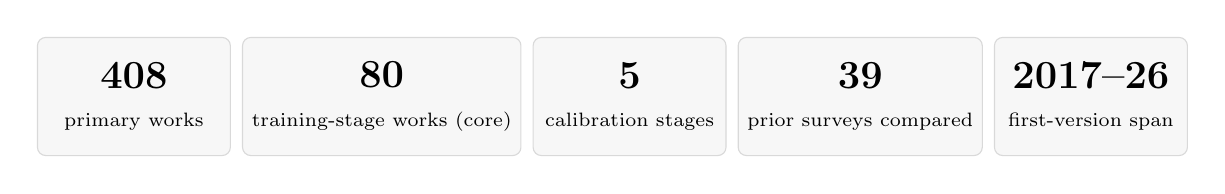
\begin{tikzpicture}
\matrix[column sep=4pt]{
\node[draw=black!15,fill=black!3,rounded corners=3pt,minimum width=2.45cm,minimum height=1.5cm,align=center] {\Large\bfseries 408\\[2pt]\scriptsize primary works}; & \node[draw=black!15,fill=black!3,rounded corners=3pt,minimum width=2.45cm,minimum height=1.5cm,align=center] {\Large\bfseries 80\\[2pt]\scriptsize training-stage works (core)}; & \node[draw=black!15,fill=black!3,rounded corners=3pt,minimum width=2.45cm,minimum height=1.5cm,align=center] {\Large\bfseries 5\\[2pt]\scriptsize calibration stages}; & \node[draw=black!15,fill=black!3,rounded corners=3pt,minimum width=2.45cm,minimum height=1.5cm,align=center] {\Large\bfseries 39\\[2pt]\scriptsize prior surveys compared}; & \node[draw=black!15,fill=black!3,rounded corners=3pt,minimum width=2.45cm,minimum height=1.5cm,align=center] {\Large\bfseries 2017--26\\[2pt]\scriptsize first-version span}; \\
};
\end{tikzpicture}\\[6pt]
\begin{tikzpicture}
\begin{axis}[xbar,bar width=10pt,width=0.84\textwidth,height=5.6cm,xmin=0,
  symbolic y coords={{X consumers and contract},{Theory and analysis},{S4 training},{S3 extra inference},{S2 prompt elicitation},{S1 post-hoc map},{S0 read-off}},ytick={{X consumers and contract},{Theory and analysis},{S4 training},{S3 extra inference},{S2 prompt elicitation},{S1 post-hoc map},{S0 read-off}},y dir=normal,
  nodes near coords,nodes near coords style={font=\footnotesize},xlabel={\footnotesize works},tick label style={font=\footnotesize},
  axis line style={black!45},xmajorgrids,grid style={black!8},enlarge x limits={upper,value=0.12}]
\addplot[fill=stS0,draw=none,bar shift=0pt] coordinates {(25,{S0 read-off})};
\addplot[fill=stS1,draw=none,bar shift=0pt] coordinates {(52,{S1 post-hoc map})};
\addplot[fill=stS2,draw=none,bar shift=0pt] coordinates {(54,{S2 prompt elicitation})};
\addplot[fill=stS3,draw=none,bar shift=0pt] coordinates {(121,{S3 extra inference})};
\addplot[fill=stS4,draw=none,bar shift=0pt] coordinates {(80,{S4 training})};
\addplot[fill=stTH,draw=none,bar shift=0pt] coordinates {(5,{Theory and analysis})};
\addplot[fill=stX,draw=none,bar shift=0pt] coordinates {(71,{X consumers and contract})};
\end{axis}
\end{tikzpicture}
\caption{\textbf{The corpus at a glance.} 408 primary works (451 references cited across the figures and tables), placed by the stage at which
calibration enters (Table~\ref{tab:definitions}); the X group holds works that consume the confidence or fix the output
contract, and the theory group holds analyses of training-stage calibration. 39 prior surveys are compared in
Table~\ref{tab:survey_compare}.}
\Description{Five stat cards (works, training-stage works, stages, prior surveys and year span) above a horizontal bar
chart of works per stage.}
\label{fig:corpus_overview}
\end{figure}

% AUTO-GENERATED by build/gen_corpus.py from literature/corpus.tsv -- do not hand-edit.
\begin{figure}[t]
\centering
\definecolor{cc0}{HTML}{1F77B4}
\definecolor{cc1}{HTML}{FF7F0E}
\definecolor{cc2}{HTML}{2CA02C}
\definecolor{cc3}{HTML}{D62728}
\definecolor{cc4}{HTML}{9467BD}
\definecolor{cc5}{HTML}{8C564B}
\definecolor{cc6}{HTML}{E377C2}
\definecolor{cc7}{HTML}{17BECF}
\definecolor{cc8}{HTML}{BCBD22}
\definecolor{cc9}{HTML}{7F7F7F}
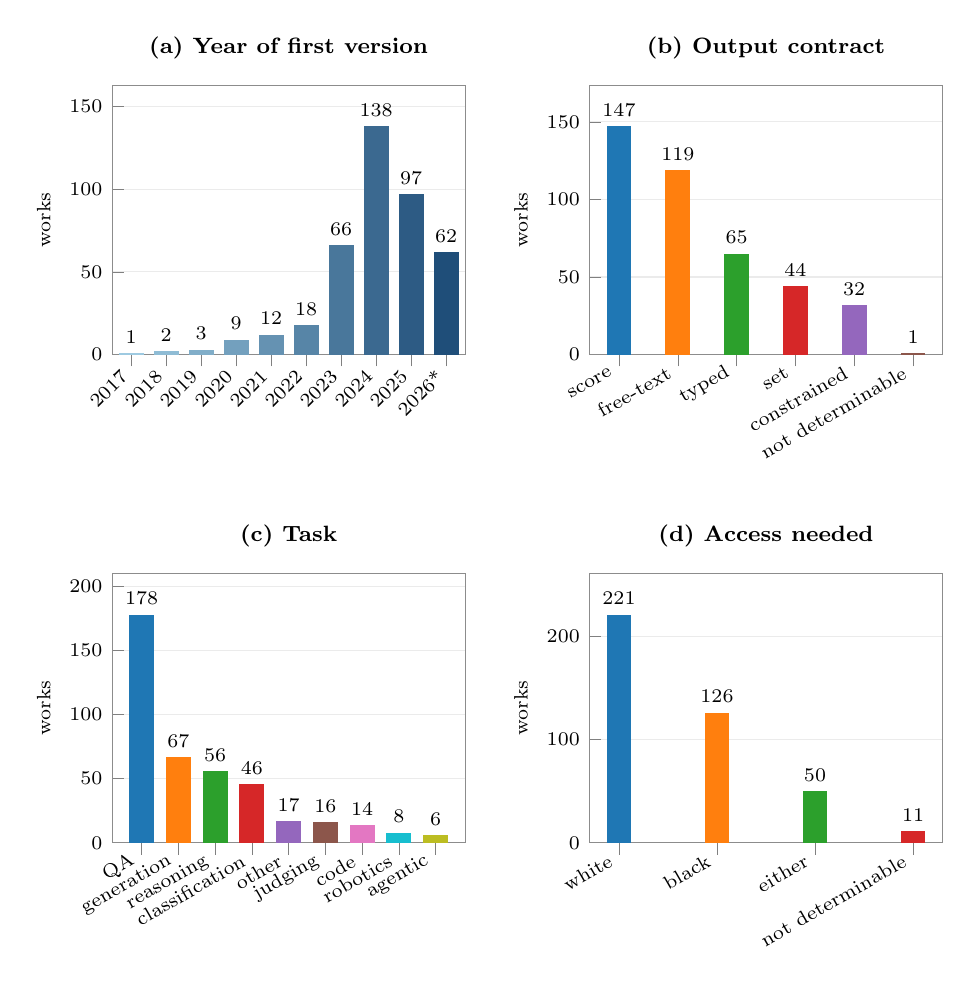
\begin{tikzpicture}
\begin{scope}\begin{axis}[ybar,bar width=9pt,width=0.5\textwidth,height=5cm,ymin=0,
  symbolic x coords={{2017},{2018},{2019},{2020},{2021},{2022},{2023},{2024},{2025},{2026*}},xtick={{2017},{2018},{2019},{2020},{2021},{2022},{2023},{2024},{2025},{2026*}},x tick label style={font=\scriptsize,rotate=45,anchor=east},
  nodes near coords,nodes near coords style={font=\scriptsize},title={\footnotesize\bfseries (a) Year of first version},
  ylabel={\scriptsize works},tick label style={font=\scriptsize},axis line style={black!45},tick pos=left,ymajorgrids,grid style={black!8},
  enlarge x limits=0.06,enlarge y limits={upper,value=0.18}]
\addplot[fill={rgb,255:red,158;green,202;blue,225},draw=none,bar shift=0pt] coordinates {({2017},1)};
\addplot[fill={rgb,255:red,143;green,188;blue,213},draw=none,bar shift=0pt] coordinates {({2018},2)};
\addplot[fill={rgb,255:red,129;green,174;blue,201},draw=none,bar shift=0pt] coordinates {({2019},3)};
\addplot[fill={rgb,255:red,115;green,160;blue,190},draw=none,bar shift=0pt] coordinates {({2020},9)};
\addplot[fill={rgb,255:red,101;green,146;blue,178},draw=none,bar shift=0pt] coordinates {({2021},12)};
\addplot[fill={rgb,255:red,87;green,133;blue,167},draw=none,bar shift=0pt] coordinates {({2022},18)};
\addplot[fill={rgb,255:red,73;green,119;blue,155},draw=none,bar shift=0pt] coordinates {({2023},66)};
\addplot[fill={rgb,255:red,59;green,105;blue,144},draw=none,bar shift=0pt] coordinates {({2024},138)};
\addplot[fill={rgb,255:red,45;green,91;blue,132},draw=none,bar shift=0pt] coordinates {({2025},97)};
\addplot[fill={rgb,255:red,31;green,78;blue,121},draw=none,bar shift=0pt] coordinates {({2026*},62)};
\end{axis}\end{scope}
\begin{scope}[xshift=0.5\textwidth]\begin{axis}[ybar,bar width=9pt,width=0.5\textwidth,height=5cm,ymin=0,
  symbolic x coords={{score},{free-text},{typed},{set},{constrained},{not determinable}},xtick={{score},{free-text},{typed},{set},{constrained},{not determinable}},x tick label style={font=\scriptsize,rotate=30,anchor=east},
  nodes near coords,nodes near coords style={font=\scriptsize},enlarge x limits=0.1,
  title={\footnotesize\bfseries (b) Output contract},ylabel={\scriptsize works},tick label style={font=\scriptsize},axis line style={black!45},tick pos=left,
  ymajorgrids,grid style={black!8},enlarge y limits={upper,value=0.18}]
\addplot[fill=cc0,draw=none,bar shift=0pt] coordinates {({score},147)};
\addplot[fill=cc1,draw=none,bar shift=0pt] coordinates {({free-text},119)};
\addplot[fill=cc2,draw=none,bar shift=0pt] coordinates {({typed},65)};
\addplot[fill=cc3,draw=none,bar shift=0pt] coordinates {({set},44)};
\addplot[fill=cc4,draw=none,bar shift=0pt] coordinates {({constrained},32)};
\addplot[fill=cc5,draw=none,bar shift=0pt] coordinates {({not determinable},1)};
\end{axis}\end{scope}
\begin{scope}[yshift=-6.2cm]\begin{axis}[ybar,bar width=9pt,width=0.5\textwidth,height=5cm,ymin=0,
  symbolic x coords={{QA},{generation},{reasoning},{classification},{other},{judging},{code},{robotics},{agentic}},xtick={{QA},{generation},{reasoning},{classification},{other},{judging},{code},{robotics},{agentic}},x tick label style={font=\scriptsize,rotate=30,anchor=east},
  nodes near coords,nodes near coords style={font=\scriptsize},enlarge x limits=0.1,
  title={\footnotesize\bfseries (c) Task},ylabel={\scriptsize works},tick label style={font=\scriptsize},axis line style={black!45},tick pos=left,
  ymajorgrids,grid style={black!8},enlarge y limits={upper,value=0.18}]
\addplot[fill=cc0,draw=none,bar shift=0pt] coordinates {({QA},178)};
\addplot[fill=cc1,draw=none,bar shift=0pt] coordinates {({generation},67)};
\addplot[fill=cc2,draw=none,bar shift=0pt] coordinates {({reasoning},56)};
\addplot[fill=cc3,draw=none,bar shift=0pt] coordinates {({classification},46)};
\addplot[fill=cc4,draw=none,bar shift=0pt] coordinates {({other},17)};
\addplot[fill=cc5,draw=none,bar shift=0pt] coordinates {({judging},16)};
\addplot[fill=cc6,draw=none,bar shift=0pt] coordinates {({code},14)};
\addplot[fill=cc7,draw=none,bar shift=0pt] coordinates {({robotics},8)};
\addplot[fill=cc8,draw=none,bar shift=0pt] coordinates {({agentic},6)};
\end{axis}\end{scope}
\begin{scope}[xshift=0.5\textwidth,yshift=-6.2cm]\begin{axis}[ybar,bar width=9pt,width=0.5\textwidth,height=5cm,ymin=0,
  symbolic x coords={{white},{black},{either},{not determinable}},xtick={{white},{black},{either},{not determinable}},x tick label style={font=\scriptsize,rotate=30,anchor=east},
  nodes near coords,nodes near coords style={font=\scriptsize},enlarge x limits=0.1,
  title={\footnotesize\bfseries (d) Access needed},ylabel={\scriptsize works},tick label style={font=\scriptsize},axis line style={black!45},tick pos=left,
  ymajorgrids,grid style={black!8},enlarge y limits={upper,value=0.18}]
\addplot[fill=cc0,draw=none,bar shift=0pt] coordinates {({white},221)};
\addplot[fill=cc1,draw=none,bar shift=0pt] coordinates {({black},126)};
\addplot[fill=cc2,draw=none,bar shift=0pt] coordinates {({either},50)};
\addplot[fill=cc3,draw=none,bar shift=0pt] coordinates {({not determinable},11)};
\end{axis}\end{scope}
\end{tikzpicture}
\caption{\textbf{Profile of the 408 corpus works} (Tables~\ref{tab:compare_s4} and~\ref{tab:landscape}). (a)~Year of first public version
(*2026 is partial); (b)~the output contract the confidence is attached to (the five contracts are defined in the caption of Table~\ref{tab:landscape}); (c)~task; (d)~the access a method needs:
white-box (logits or weights), black-box (text only) or either. ``not determinable'' marks a value that could not be determined from the paper.}
\Description{Four bar charts describing the corpus: works per year, per output contract, per task and per access level.}
\label{fig:corpus_dist}
\end{figure}

% AUTO-GENERATED by build/gen_corpus.py from literature/corpus.tsv -- do not hand-edit.
\begin{figure}[t]
\centering
\begin{tikzpicture}
\begin{axis}[width=\textwidth,height=6.6cm,xmin=2016.6,xmax=2026.4,ymin=0,
  xtick={2017,2018,2019,2020,2021,2022,2023,2024,2025,2026},xticklabels={2017,2018,2019,2020,2021,2022,2023,2024,2025,2026*},
  ylabel={works in the corpus},xlabel={year of first public version},grid=major,grid style={black!8},
  legend style={at={(0.02,0.98)},anchor=north west,font=\footnotesize,draw=black!20,fill=white,fill opacity=0.9,text opacity=1},
  tick label style={font=\footnotesize},label style={font=\footnotesize},axis line style={black!50}]
\addplot[color=stS0,line width=1.4pt,mark=*,mark size=1.8pt] coordinates {(2017,0) (2018,1) (2019,0) (2020,2) (2021,2) (2022,6) (2023,4) (2024,6) (2025,1)}; \addlegendentry{S0 read-off}
\addplot[color=stS0,line width=1.4pt,dashed,mark=*,mark size=1.8pt,forget plot] coordinates {(2025,1) (2026,3)};
\addplot[color=stS1,line width=1.4pt,mark=*,mark size=1.8pt] coordinates {(2017,1) (2018,0) (2019,3) (2020,1) (2021,5) (2022,3) (2023,11) (2024,19) (2025,6)}; \addlegendentry{S1 post-hoc map}
\addplot[color=stS1,line width=1.4pt,dashed,mark=*,mark size=1.8pt,forget plot] coordinates {(2025,6) (2026,3)};
\addplot[color=stS2,line width=1.4pt,mark=*,mark size=1.8pt] coordinates {(2017,0) (2018,0) (2019,0) (2020,0) (2021,0) (2022,1) (2023,7) (2024,22) (2025,15)}; \addlegendentry{S2 prompt elicitation}
\addplot[color=stS2,line width=1.4pt,dashed,mark=*,mark size=1.8pt,forget plot] coordinates {(2025,15) (2026,9)};
\addplot[color=stS3,line width=1.4pt,mark=*,mark size=1.8pt] coordinates {(2017,0) (2018,1) (2019,0) (2020,3) (2021,4) (2022,4) (2023,27) (2024,44) (2025,29)}; \addlegendentry{S3 extra inference}
\addplot[color=stS3,line width=1.4pt,dashed,mark=*,mark size=1.8pt,forget plot] coordinates {(2025,29) (2026,9)};
\addplot[color=stS4,line width=1.4pt,mark=*,mark size=1.8pt] coordinates {(2017,0) (2018,0) (2019,0) (2020,2) (2021,0) (2022,1) (2023,2) (2024,22) (2025,25)}; \addlegendentry{S4 training}
\addplot[color=stS4,line width=1.4pt,dashed,mark=*,mark size=1.8pt,forget plot] coordinates {(2025,25) (2026,28)};
\addplot[color=stX,line width=1.4pt,mark=*,mark size=1.8pt] coordinates {(2017,0) (2018,0) (2019,0) (2020,1) (2021,1) (2022,3) (2023,13) (2024,25) (2025,18)}; \addlegendentry{X consumers and contract}
\addplot[color=stX,line width=1.4pt,dashed,mark=*,mark size=1.8pt,forget plot] coordinates {(2025,18) (2026,10)};
\end{axis}
\end{tikzpicture}
\caption{\textbf{Works per stage per year} (Tables~\ref{tab:compare_s4} and~\ref{tab:landscape}). 75 of the 80 training-stage (S4) works
appeared in 2024 to 2026 (94\%), against 166 of the 252 works at stages S0 to S3 (66\%) over the same years.
*2026 covers January to September, drawn dashed. The 5 theory and analysis works are not plotted.}
\Description{A line chart of corpus works per year from 2017 to 2026, one coloured line per stage. The
training-stage line rises steeply in the last three years; the last segment of each line is dashed because the final year is
partial.}
\label{fig:stage_trend}
\end{figure}


Figures~\ref{fig:method_gallery} and~\ref{fig:results_gallery} show, stage by stage, how the papers
themselves depict their methods and their results. Panels are chosen by a fixed rule and reproduced only
from papers whose licence permits reuse; the rule, and each panel's source figure, page and licence, are
in Table~\ref{tab:panel_provenance} (Appendix~\ref{app:provenance}).

% AUTO-GENERATED by build/gallery.py compile (pipeline tool gen_compilation_figure.py --fit)
% AUTO-GENERATED by tools/gen_compilation_figure.py -- vector TikZ, main-body, hyperlinked.
\begin{figure*}[tp]
\centering
\resizebox{\textwidth}{!}{%
\begin{tikzpicture}[x=1cm,y=1cm]
\definecolor{c355475}{HTML}{355475}
\definecolor{cAB5D10}{HTML}{AB5D10}
\definecolor{c3A7134}{HTML}{3A7134}
\definecolor{c7C5471}{HTML}{7C5471}
\definecolor{c9F3C3C}{HTML}{9F3C3C}
\fill[black!88] (0,0) rectangle (13.800,-0.580);
\node[anchor=west,text=white,font=\small\bfseries,inner sep=0] at (0.14,-0.290) {How confidence is produced and used, by stage};
\fill[c355475] (0,-0.580) rectangle (13.800,-1.080);
\node[anchor=west,text=white,font=\footnotesize\bfseries,inner sep=0] at (0.14,-0.830) {S1 post-hoc map};
\node[anchor=north west,inner sep=0] at (2.816,-1.150) {\href{https://arxiv.org/abs/2607.16799}{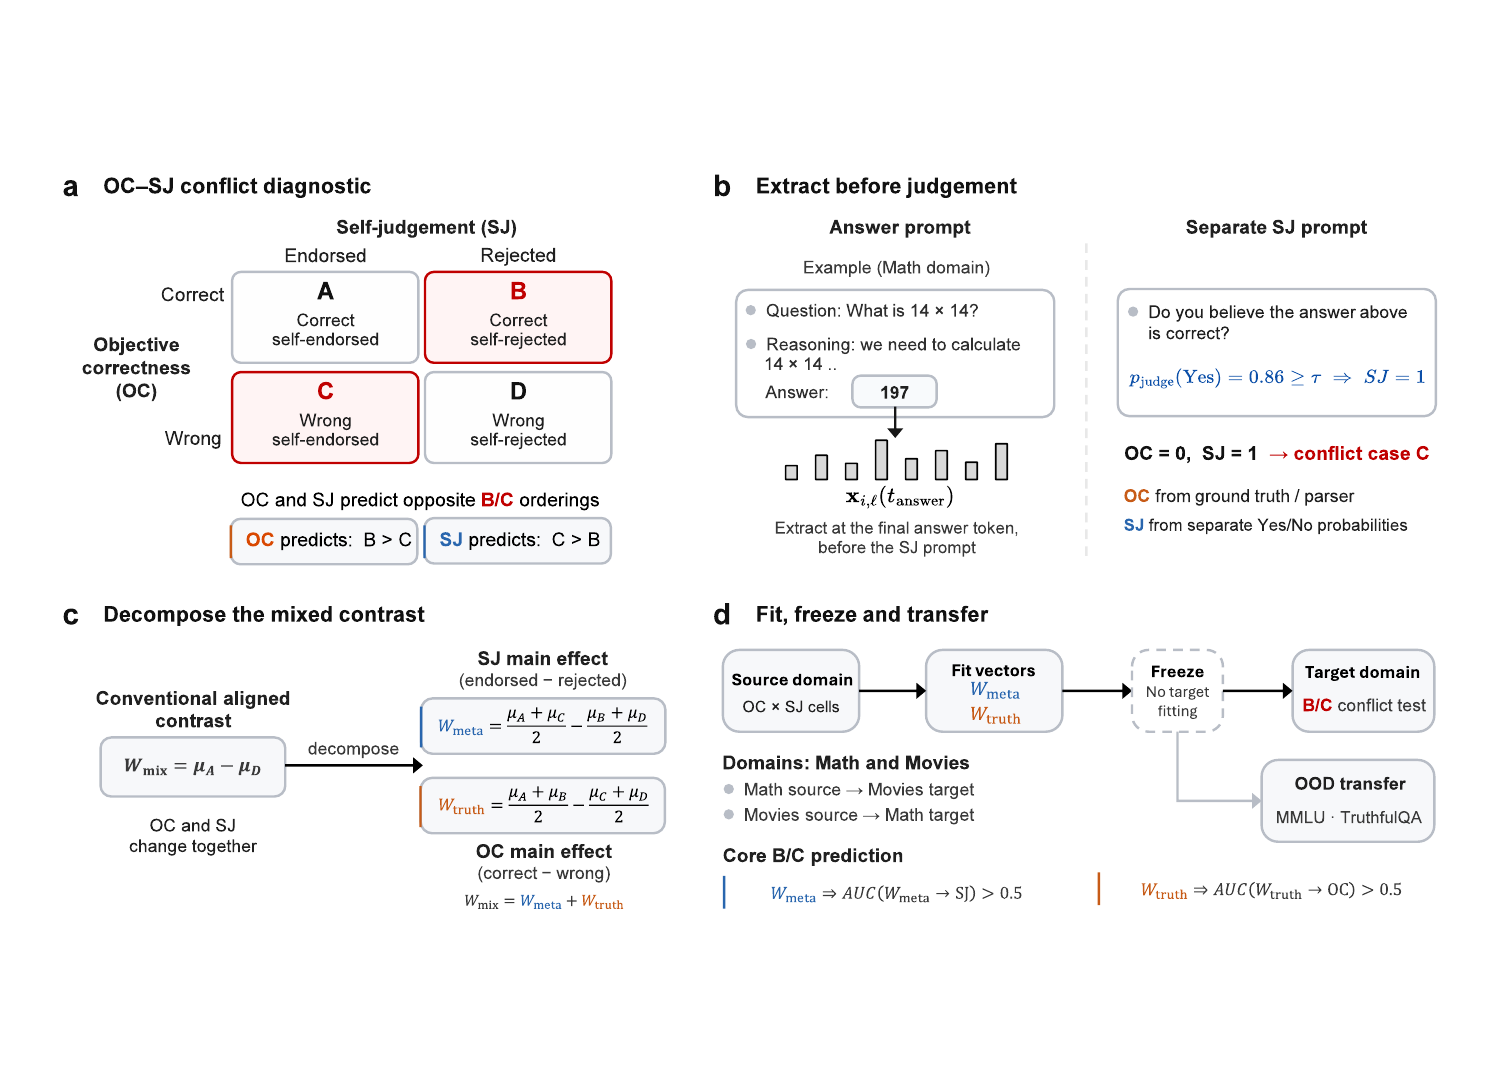
\includegraphics[width=2.676cm]{figures/img/method_gallery/tile_0.png}}};
\draw[black!35,line width=0.35pt] (2.816,-1.150) rectangle (5.492,-3.077);
\node[anchor=north west,text=ACMDarkBlue,font=\tiny\bfseries,inner sep=0] at (2.846,-3.107) {\href{https://arxiv.org/abs/2607.16799}{\adjustbox{max width=2.616cm}{Lu 2026}}};
\node[anchor=north west,text=black!60,font=\tiny,inner sep=0] at (2.846,-3.312) {\href{https://arxiv.org/abs/2607.16799}{Fig. 1, p.~2}};
\node[anchor=north west,inner sep=0] at (5.562,-1.150) {\href{https://arxiv.org/abs/2601.04277}{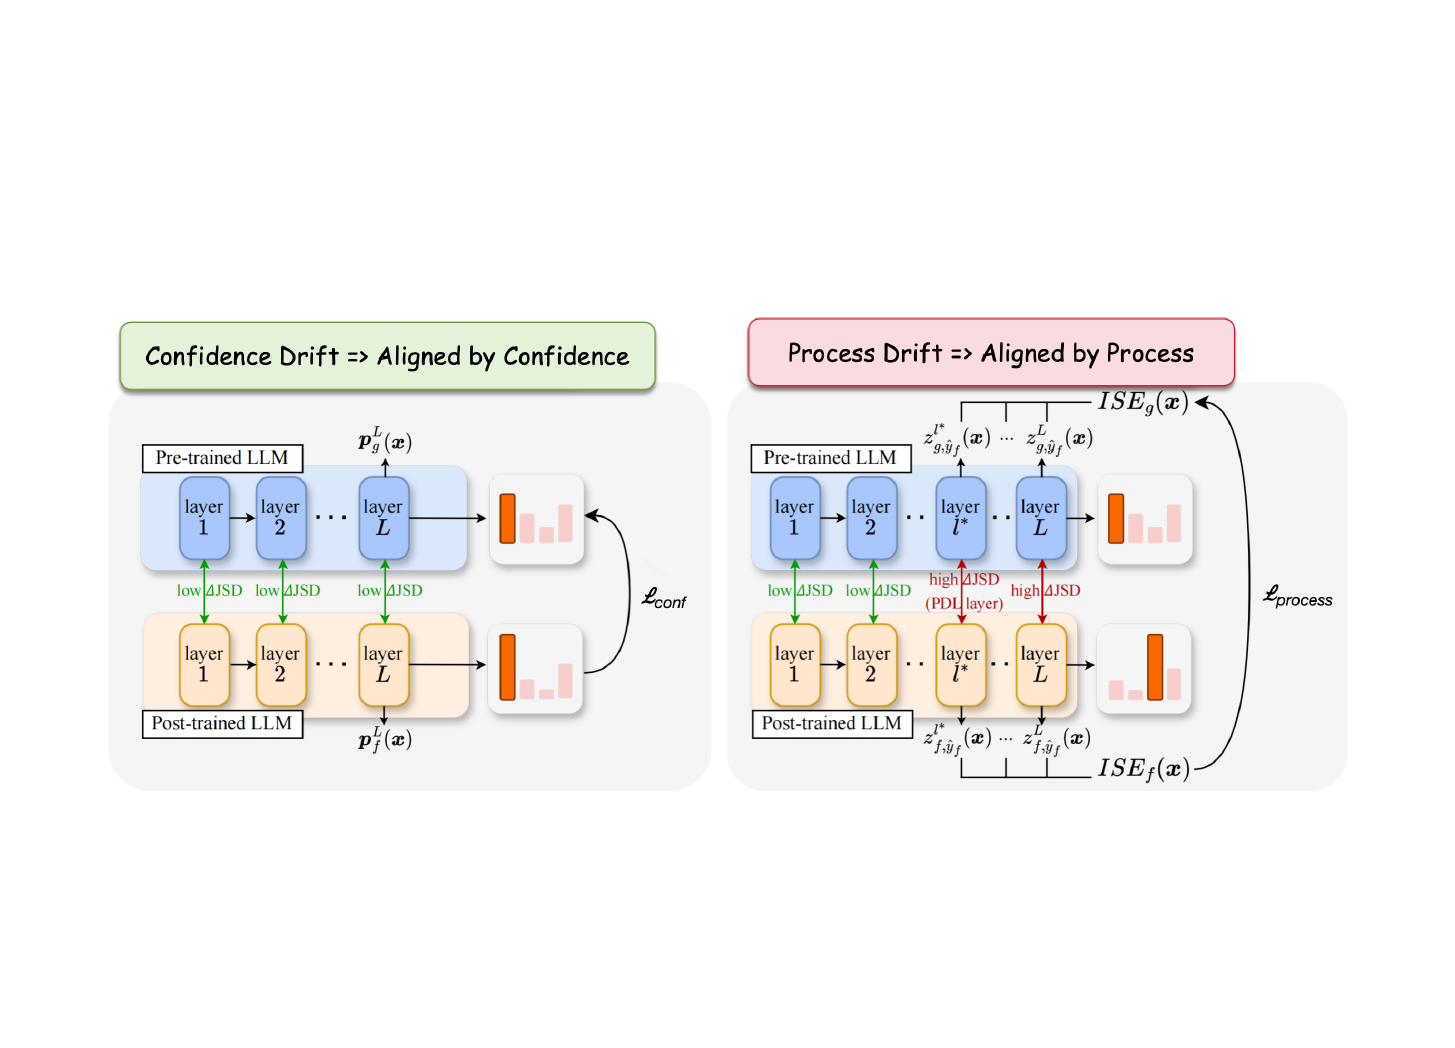
\includegraphics[width=2.676cm]{figures/img/method_gallery/tile_1.png}}};
\draw[black!35,line width=0.35pt] (5.562,-1.150) rectangle (8.238,-3.077);
\node[anchor=north west,text=ACMDarkBlue,font=\tiny\bfseries,inner sep=0] at (5.592,-3.107) {\href{https://arxiv.org/abs/2601.04277}{\adjustbox{max width=2.616cm}{Luo et al. 2026}}};
\node[anchor=north west,text=black!60,font=\tiny,inner sep=0] at (5.592,-3.312) {\href{https://arxiv.org/abs/2601.04277}{Fig. 1, p.~2}};
\node[anchor=north west,inner sep=0] at (8.308,-1.150) {\href{https://arxiv.org/abs/2505.23783}{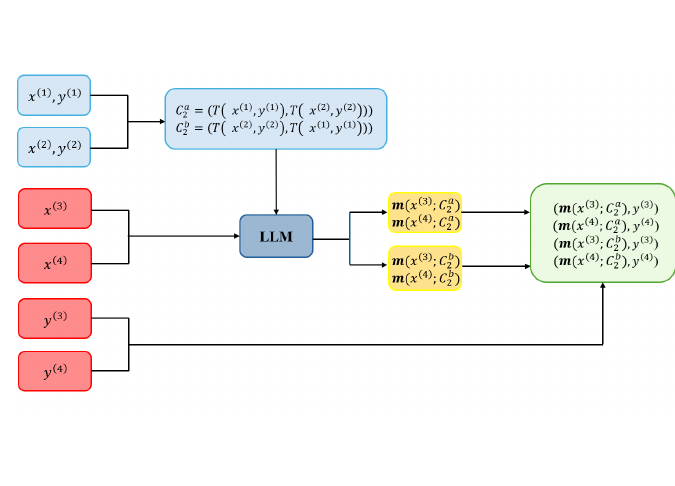
\includegraphics[width=2.676cm]{figures/img/method_gallery/tile_2.png}}};
\draw[black!35,line width=0.35pt] (8.308,-1.150) rectangle (10.984,-3.077);
\node[anchor=north west,text=ACMDarkBlue,font=\tiny\bfseries,inner sep=0] at (8.338,-3.107) {\href{https://arxiv.org/abs/2505.23783}{\adjustbox{max width=2.616cm}{Gundem et al. 2025}}};
\node[anchor=north west,text=black!60,font=\tiny,inner sep=0] at (8.338,-3.312) {\href{https://arxiv.org/abs/2505.23783}{Fig. 2, p.~5}};
\fill[cAB5D10] (0,-3.567) rectangle (13.800,-4.067);
\node[anchor=west,text=white,font=\footnotesize\bfseries,inner sep=0] at (0.14,-3.817) {S2 prompt elicitation};
\node[anchor=north west,inner sep=0] at (4.189,-4.137) {\href{https://arxiv.org/abs/2606.17234}{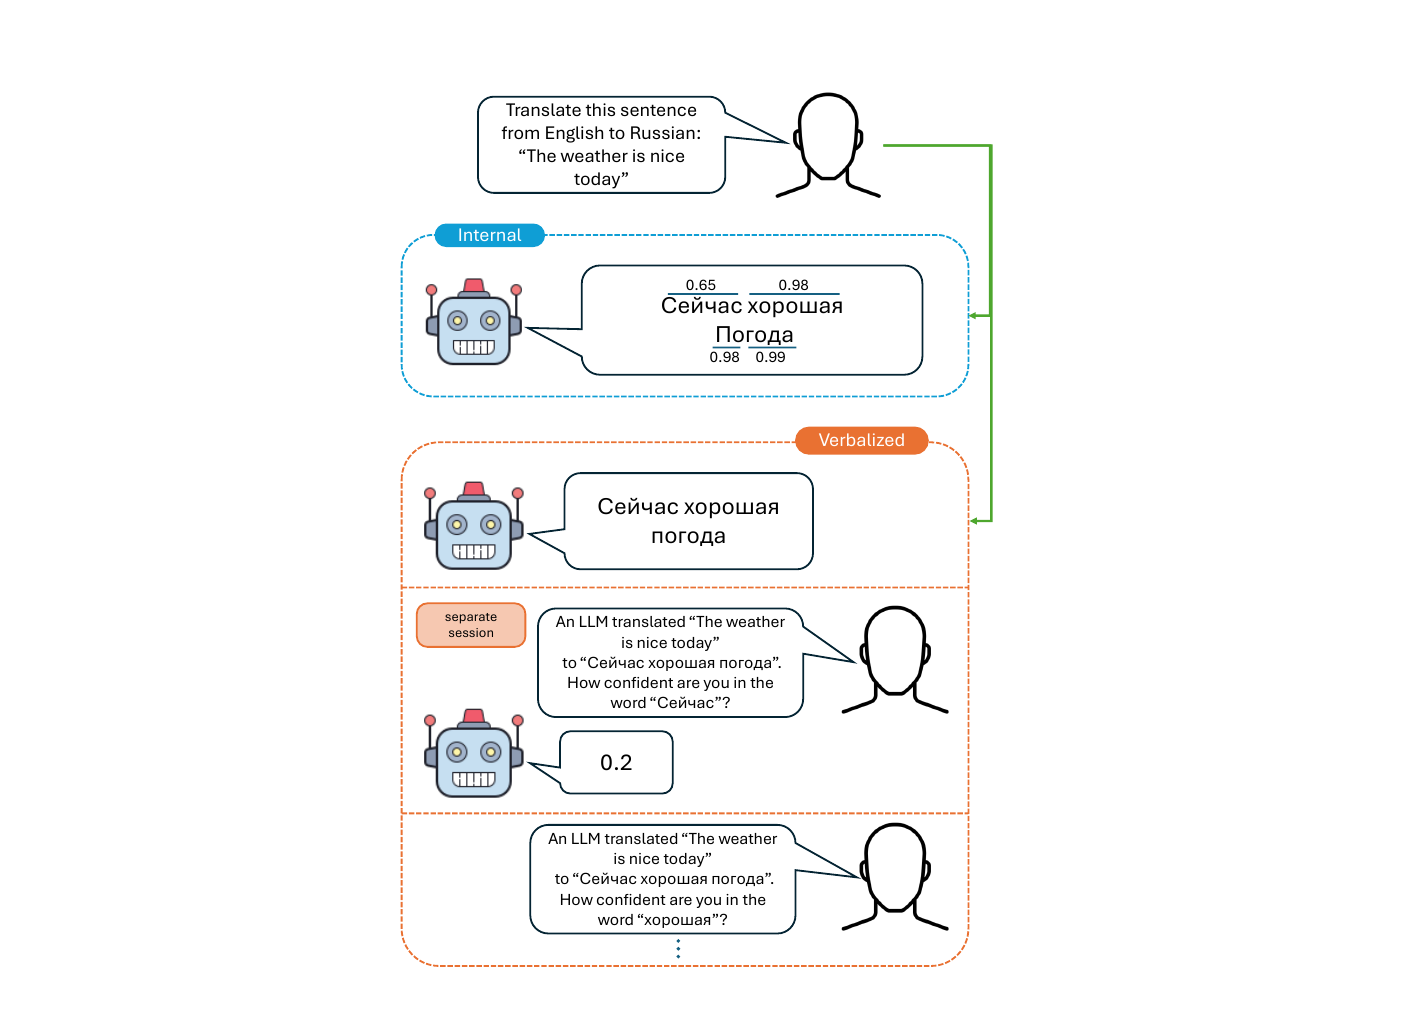
\includegraphics[width=2.676cm]{figures/img/method_gallery/tile_3.png}}};
\draw[black!35,line width=0.35pt] (4.189,-4.137) rectangle (6.865,-6.063);
\node[anchor=north west,text=ACMDarkBlue,font=\tiny\bfseries,inner sep=0] at (4.219,-6.093) {\href{https://arxiv.org/abs/2606.17234}{\adjustbox{max width=2.616cm}{Marashian et al. 2026}}};
\node[anchor=north west,text=black!60,font=\tiny,inner sep=0] at (4.219,-6.298) {\href{https://arxiv.org/abs/2606.17234}{Fig. 1, p.~1}};
\node[anchor=north west,inner sep=0] at (6.935,-4.137) {\href{https://arxiv.org/abs/2405.16282}{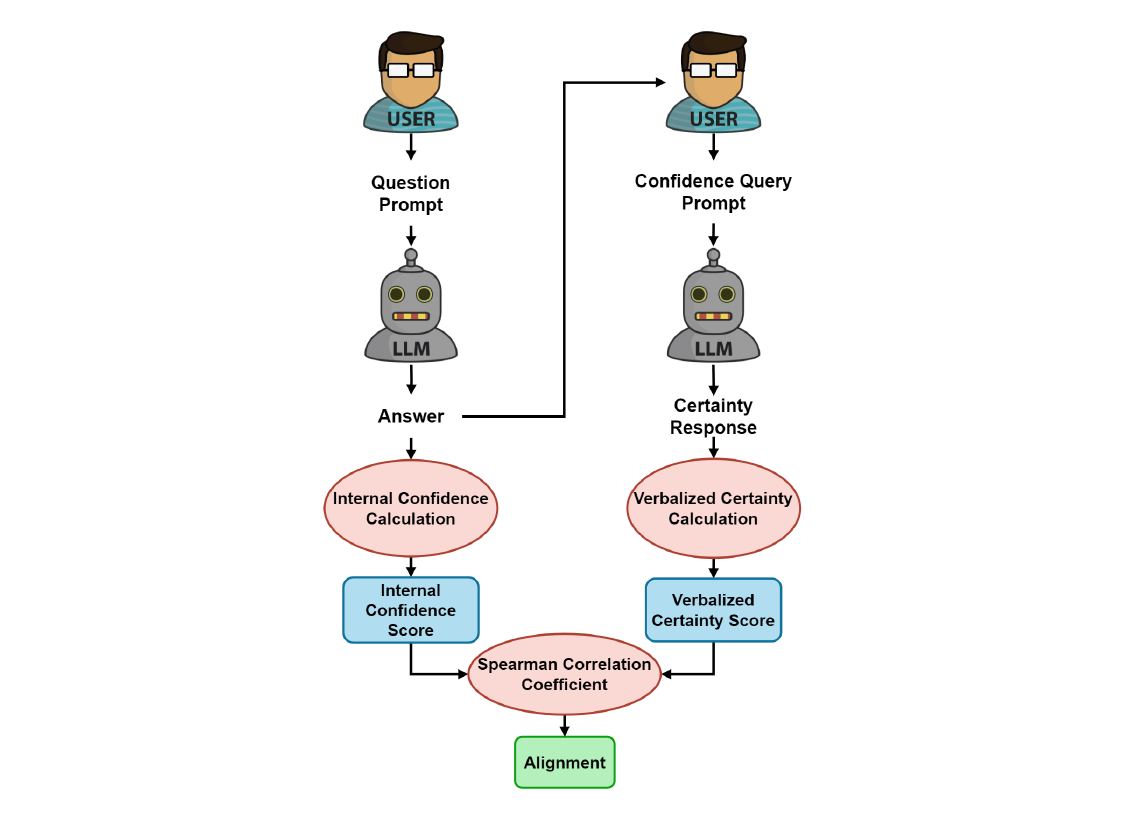
\includegraphics[width=2.676cm]{figures/img/method_gallery/tile_4.png}}};
\draw[black!35,line width=0.35pt] (6.935,-4.137) rectangle (9.611,-6.063);
\node[anchor=north west,text=ACMDarkBlue,font=\tiny\bfseries,inner sep=0] at (6.965,-6.093) {\href{https://arxiv.org/abs/2405.16282}{\adjustbox{max width=2.616cm}{Kumar et al. 2024}}};
\node[anchor=north west,text=black!60,font=\tiny,inner sep=0] at (6.965,-6.298) {\href{https://arxiv.org/abs/2405.16282}{Fig. 1, p.~1}};
\fill[c3A7134] (0,-6.553) rectangle (13.800,-7.053);
\node[anchor=west,text=white,font=\footnotesize\bfseries,inner sep=0] at (0.14,-6.803) {S3 extra inference};
\node[anchor=north west,inner sep=0] at (2.816,-7.123) {\href{https://arxiv.org/abs/2505.09427}{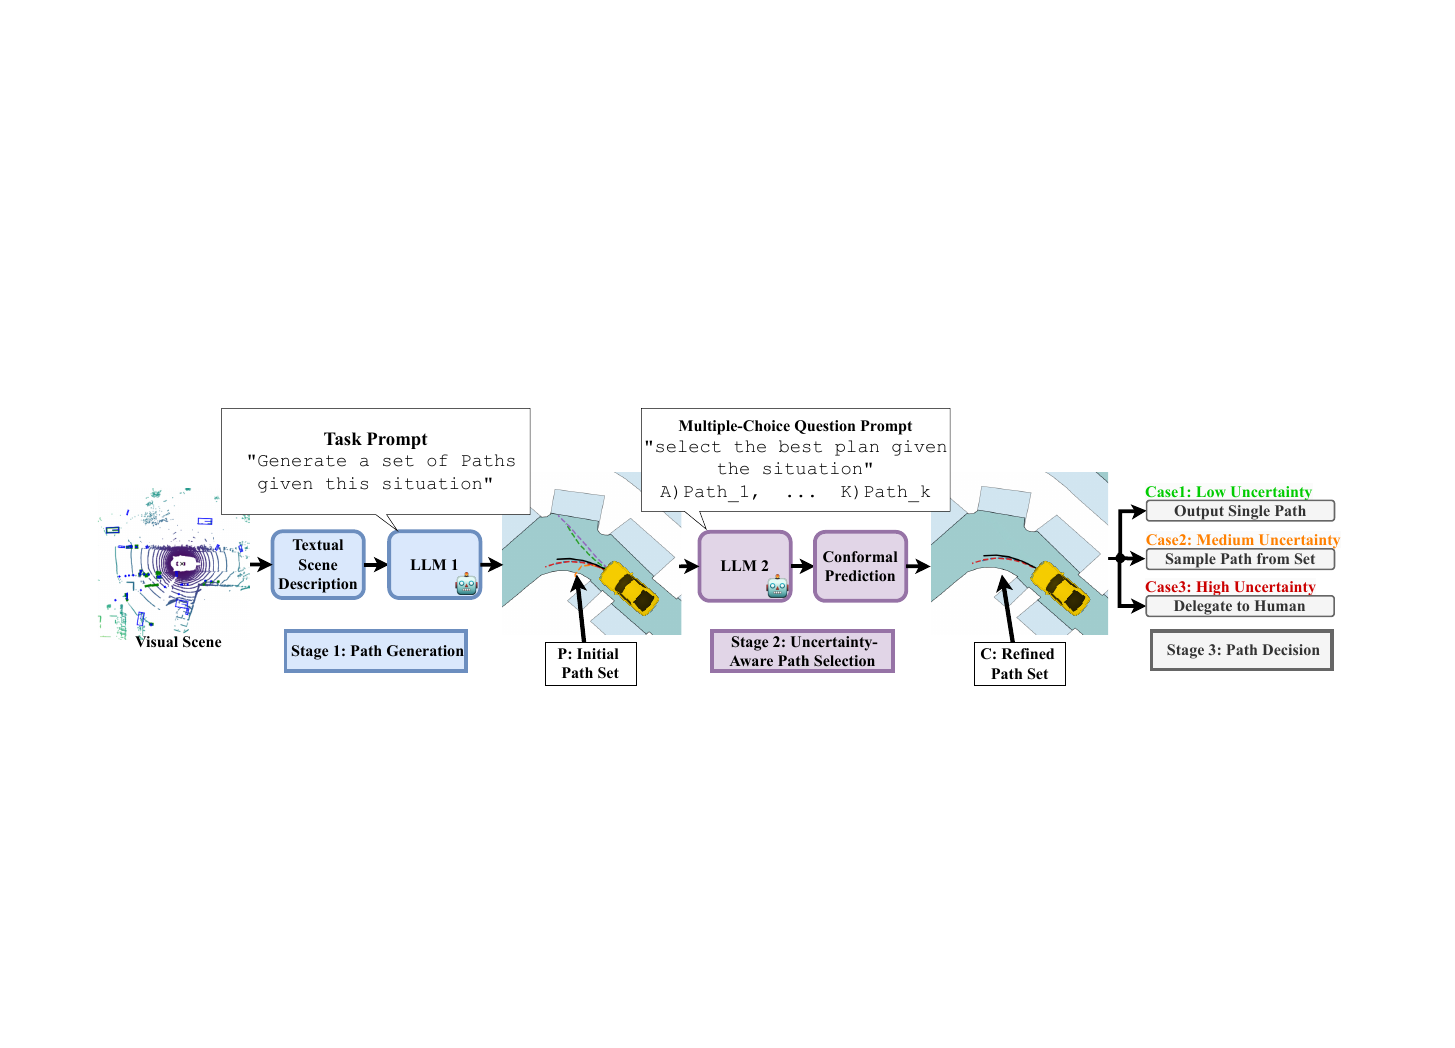
\includegraphics[width=2.676cm]{figures/img/method_gallery/tile_5.png}}};
\draw[black!35,line width=0.35pt] (2.816,-7.123) rectangle (5.492,-9.050);
\node[anchor=north west,text=ACMDarkBlue,font=\tiny\bfseries,inner sep=0] at (2.846,-9.080) {\href{https://arxiv.org/abs/2505.09427}{\adjustbox{max width=2.616cm}{Doula et al. 2025}}};
\node[anchor=north west,text=black!60,font=\tiny,inner sep=0] at (2.846,-9.285) {\href{https://arxiv.org/abs/2505.09427}{Fig. 1, p.~3}};
\node[anchor=north west,inner sep=0] at (5.562,-7.123) {\href{https://arxiv.org/abs/2305.13281}{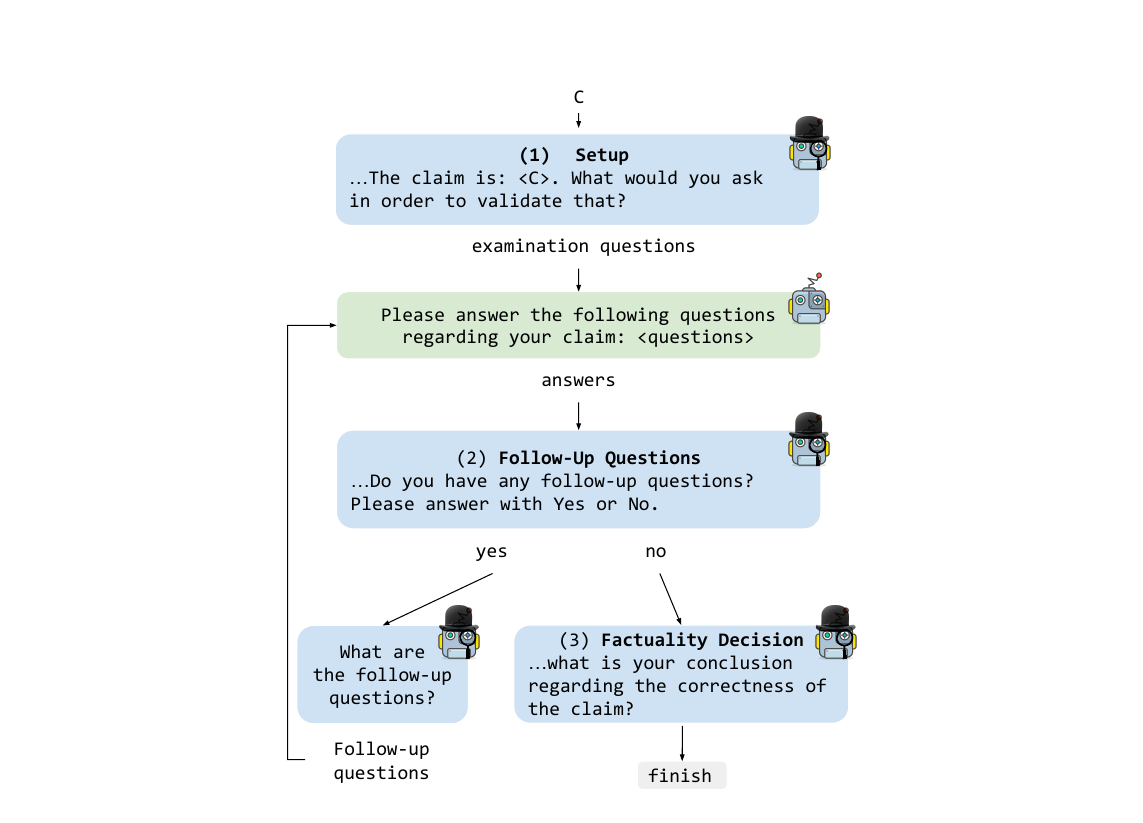
\includegraphics[width=2.676cm]{figures/img/method_gallery/tile_6.png}}};
\draw[black!35,line width=0.35pt] (5.562,-7.123) rectangle (8.238,-9.050);
\node[anchor=north west,text=ACMDarkBlue,font=\tiny\bfseries,inner sep=0] at (5.592,-9.080) {\href{https://arxiv.org/abs/2305.13281}{\adjustbox{max width=2.616cm}{Cohen et al. 2023}}};
\node[anchor=north west,text=black!60,font=\tiny,inner sep=0] at (5.592,-9.285) {\href{https://arxiv.org/abs/2305.13281}{Fig. 2, p.~3}};
\node[anchor=north west,inner sep=0] at (8.308,-7.123) {\href{https://arxiv.org/abs/2502.20285}{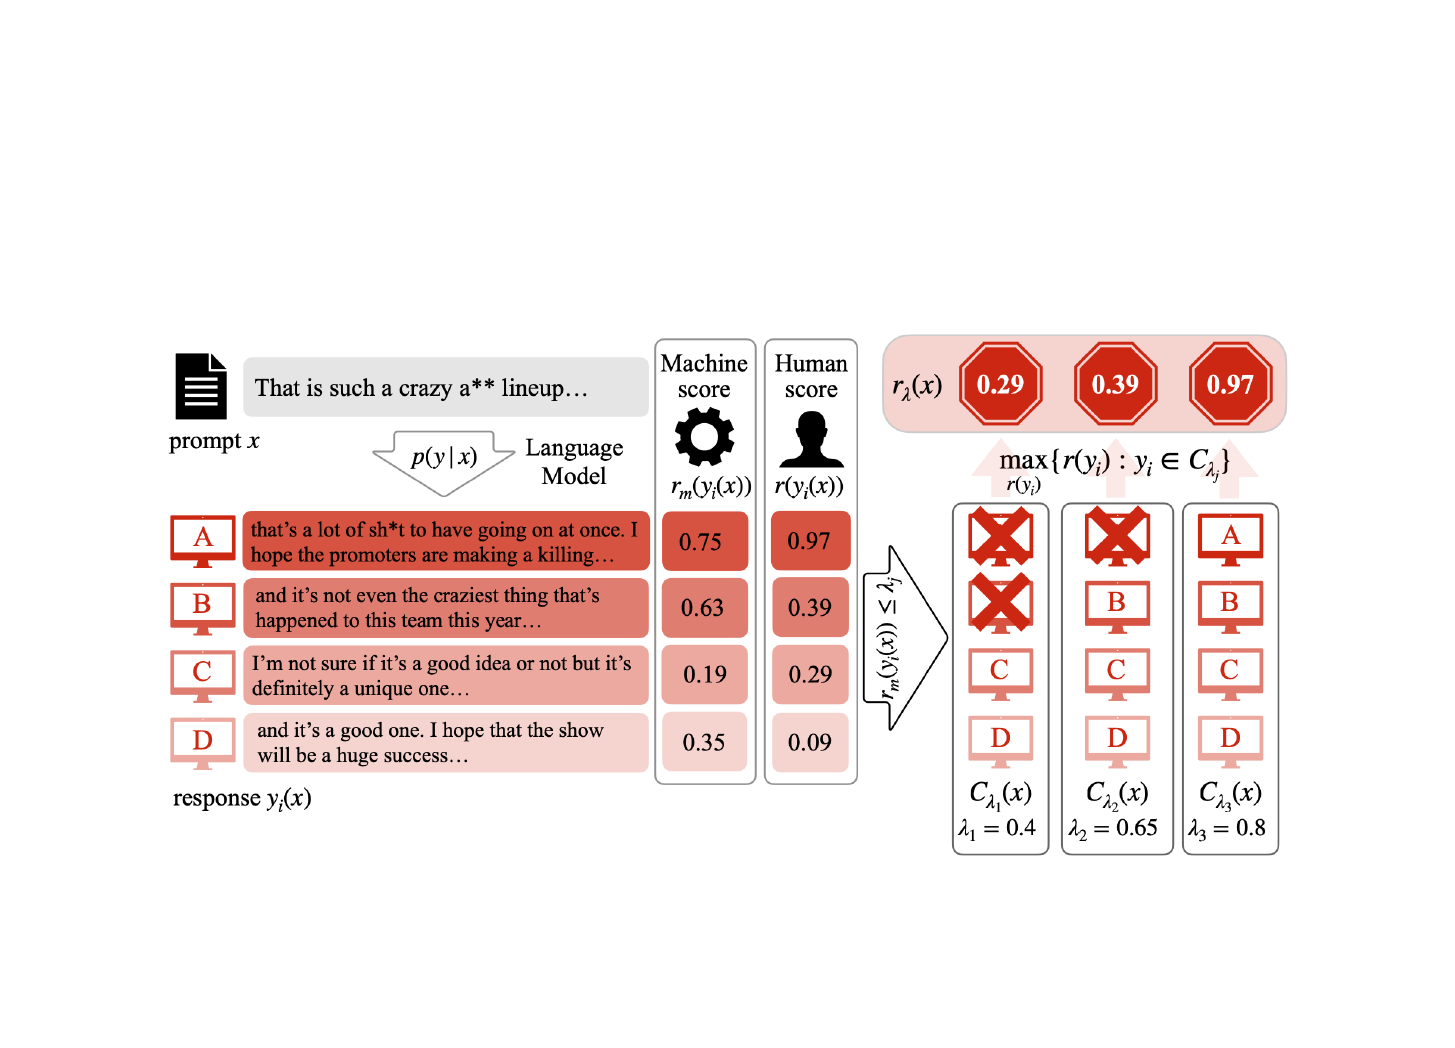
\includegraphics[width=2.676cm]{figures/img/method_gallery/tile_7.png}}};
\draw[black!35,line width=0.35pt] (8.308,-7.123) rectangle (10.984,-9.050);
\node[anchor=north west,text=ACMDarkBlue,font=\tiny\bfseries,inner sep=0] at (8.338,-9.080) {\href{https://arxiv.org/abs/2502.20285}{\adjustbox{max width=2.616cm}{Chen et al. 2025b}}};
\node[anchor=north west,text=black!60,font=\tiny,inner sep=0] at (8.338,-9.285) {\href{https://arxiv.org/abs/2502.20285}{Fig. 3, p.~8}};
\fill[c7C5471] (0,-9.540) rectangle (13.800,-10.040);
\node[anchor=west,text=white,font=\footnotesize\bfseries,inner sep=0] at (0.14,-9.790) {S4 training};
\node[anchor=north west,inner sep=0] at (2.816,-10.110) {\href{https://arxiv.org/abs/2607.01612}{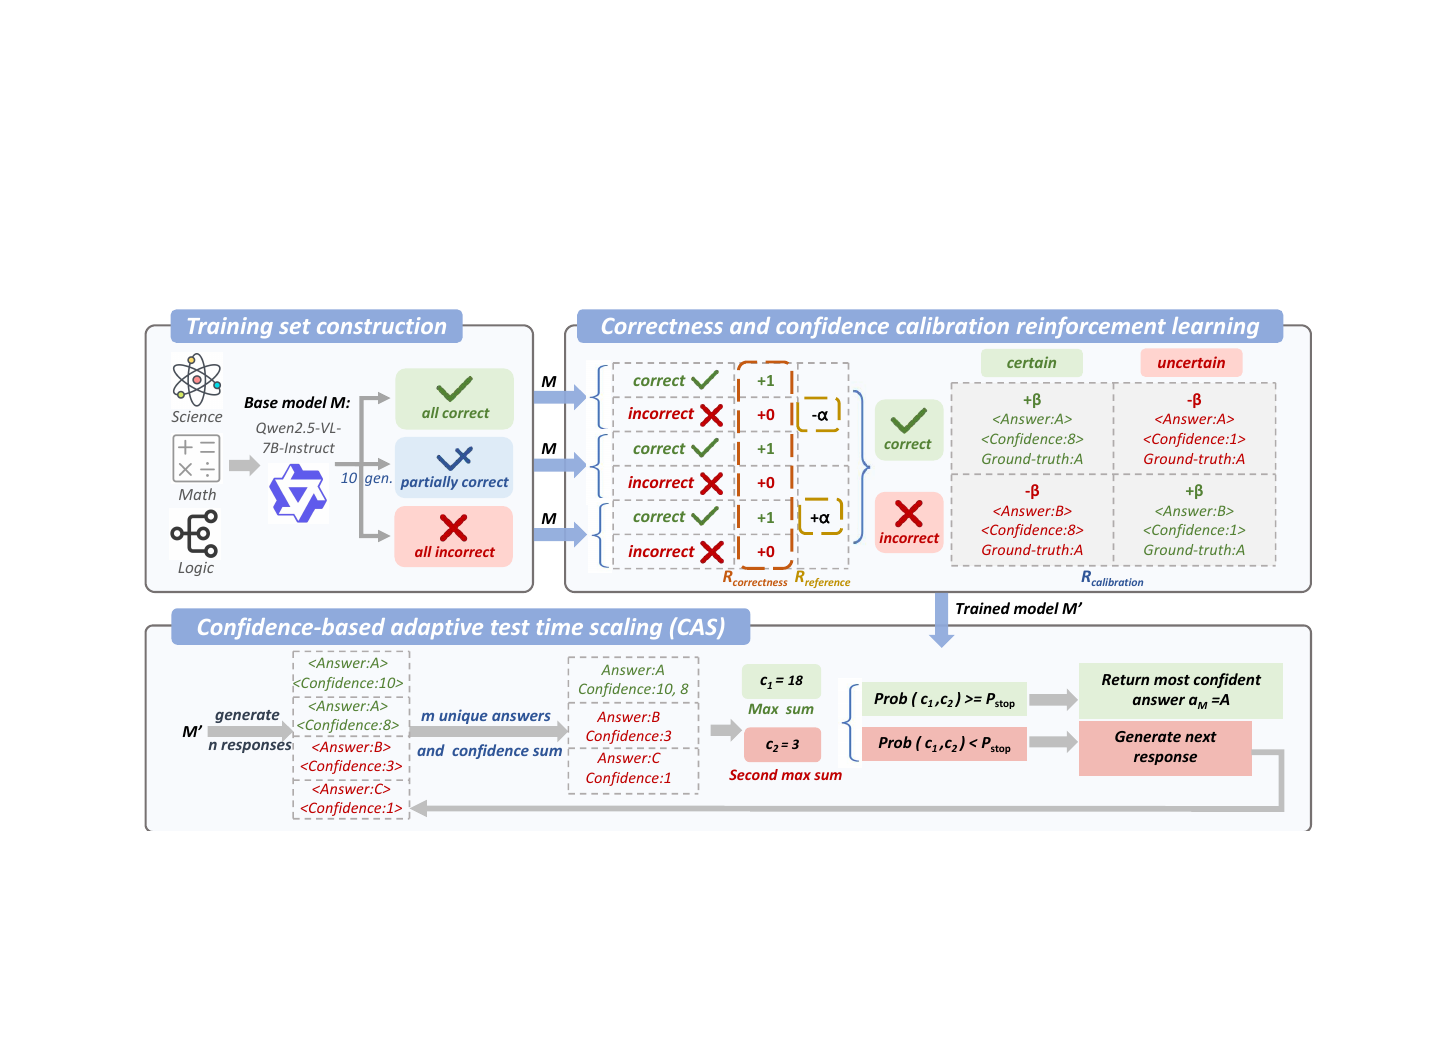
\includegraphics[width=2.676cm]{figures/img/method_gallery/tile_8.png}}};
\draw[black!35,line width=0.35pt] (2.816,-10.110) rectangle (5.492,-12.037);
\node[anchor=north west,text=ACMDarkBlue,font=\tiny\bfseries,inner sep=0] at (2.846,-12.067) {\href{https://arxiv.org/abs/2607.01612}{\adjustbox{max width=2.616cm}{Yang et al. 2026b}}};
\node[anchor=north west,text=black!60,font=\tiny,inner sep=0] at (2.846,-12.272) {\href{https://arxiv.org/abs/2607.01612}{Fig. 1, p.~3}};
\node[anchor=north west,inner sep=0] at (5.562,-10.110) {\href{https://arxiv.org/abs/2604.05306}{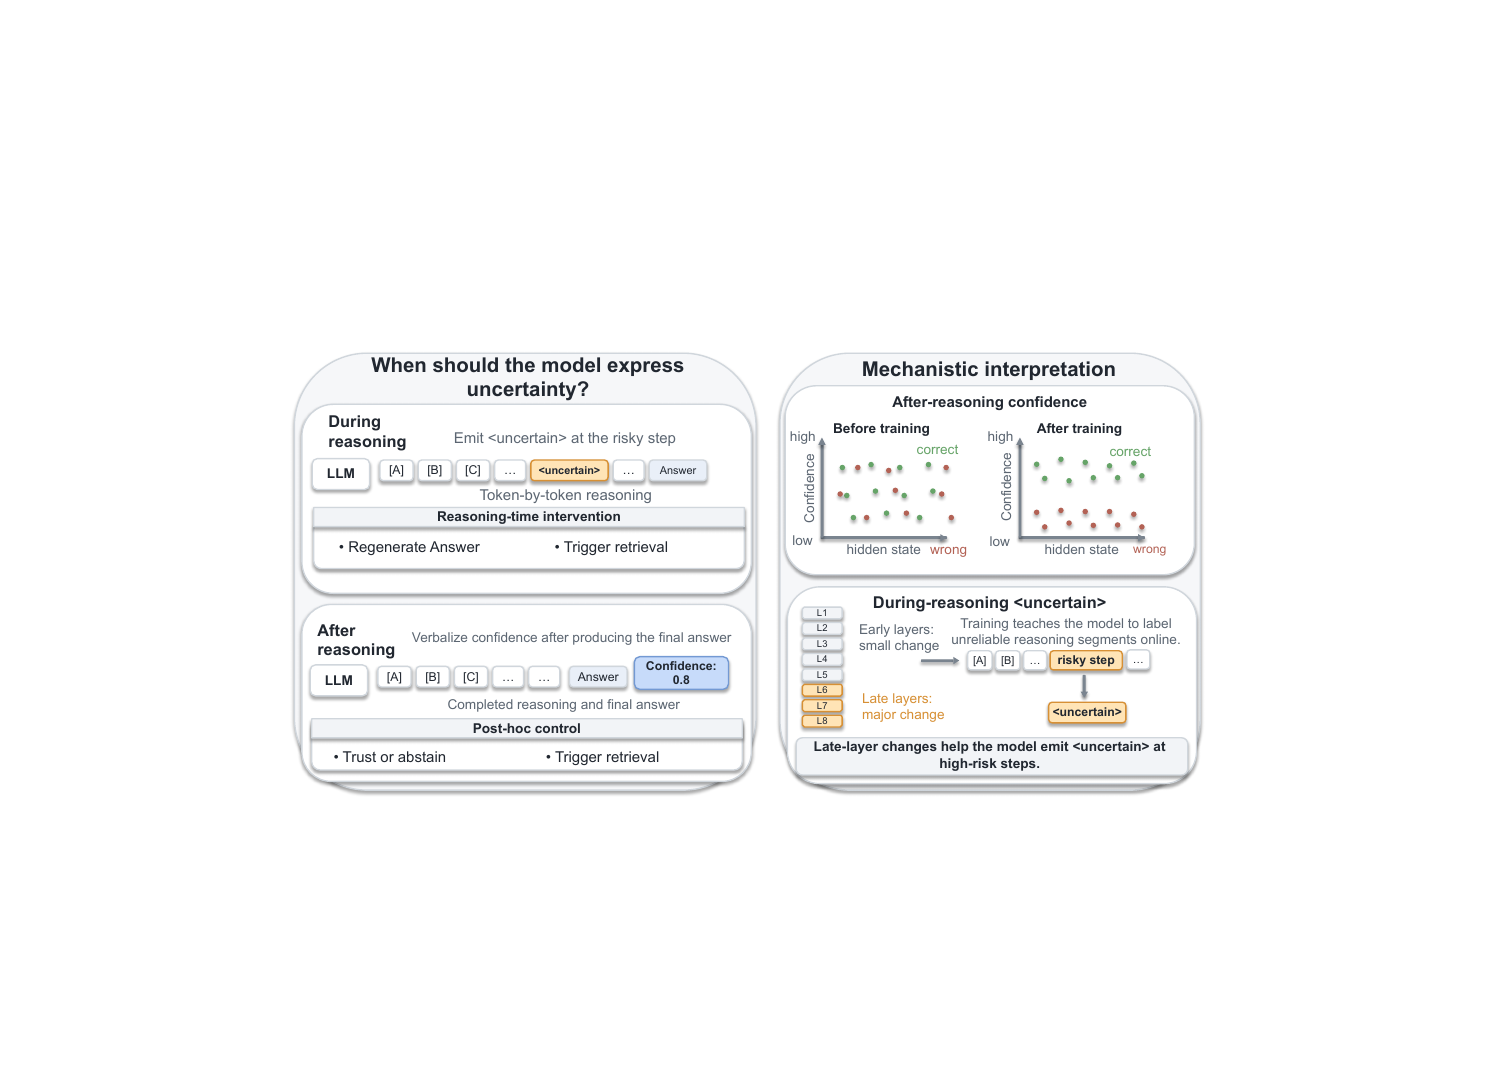
\includegraphics[width=2.676cm]{figures/img/method_gallery/tile_9.png}}};
\draw[black!35,line width=0.35pt] (5.562,-10.110) rectangle (8.238,-12.037);
\node[anchor=north west,text=ACMDarkBlue,font=\tiny\bfseries,inner sep=0] at (5.592,-12.067) {\href{https://arxiv.org/abs/2604.05306}{\adjustbox{max width=2.616cm}{Guo et al. 2026}}};
\node[anchor=north west,text=black!60,font=\tiny,inner sep=0] at (5.592,-12.272) {\href{https://arxiv.org/abs/2604.05306}{Fig. 1, p.~2}};
\node[anchor=north west,inner sep=0] at (8.308,-10.110) {\href{https://arxiv.org/abs/2604.22779}{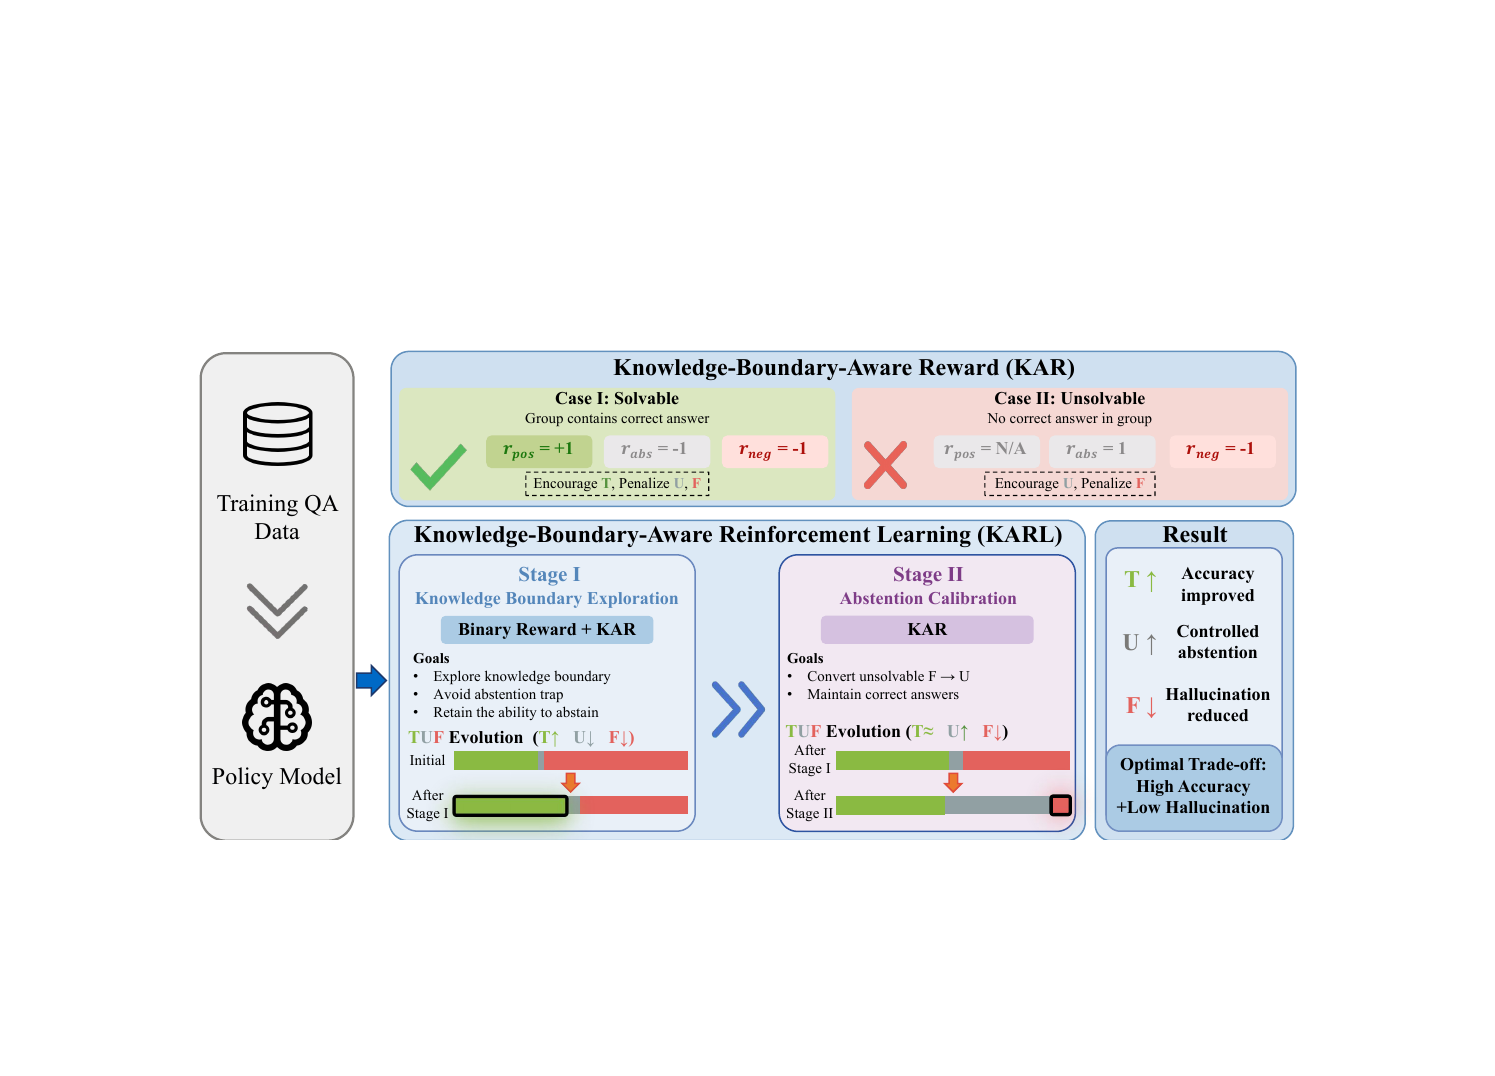
\includegraphics[width=2.676cm]{figures/img/method_gallery/tile_10.png}}};
\draw[black!35,line width=0.35pt] (8.308,-10.110) rectangle (10.984,-12.037);
\node[anchor=north west,text=ACMDarkBlue,font=\tiny\bfseries,inner sep=0] at (8.338,-12.067) {\href{https://arxiv.org/abs/2604.22779}{\adjustbox{max width=2.616cm}{Gao et al. 2026}}};
\node[anchor=north west,text=black!60,font=\tiny,inner sep=0] at (8.338,-12.272) {\href{https://arxiv.org/abs/2604.22779}{Fig. 4, p.~4}};
\fill[c9F3C3C] (0,-12.527) rectangle (13.800,-13.027);
\node[anchor=west,text=white,font=\footnotesize\bfseries,inner sep=0] at (0.14,-12.777) {X consumers and contract};
\node[anchor=north west,inner sep=0] at (2.816,-13.097) {\href{https://arxiv.org/abs/2505.04016}{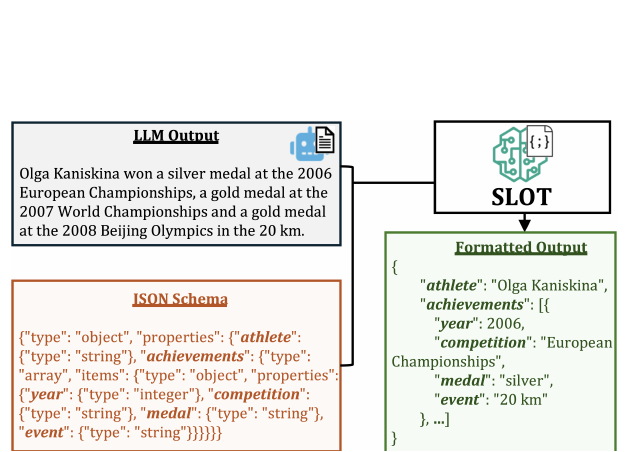
\includegraphics[width=2.676cm]{figures/img/method_gallery/tile_11.png}}};
\draw[black!35,line width=0.35pt] (2.816,-13.097) rectangle (5.492,-15.024);
\node[anchor=north west,text=ACMDarkBlue,font=\tiny\bfseries,inner sep=0] at (2.846,-15.054) {\href{https://arxiv.org/abs/2505.04016}{\adjustbox{max width=2.616cm}{Wang et al. 2025e}}};
\node[anchor=north west,text=black!60,font=\tiny,inner sep=0] at (2.846,-15.259) {\href{https://arxiv.org/abs/2505.04016}{Fig. 1, p.~1}};
\node[anchor=north west,inner sep=0] at (5.562,-13.097) {\href{https://arxiv.org/abs/2509.21837}{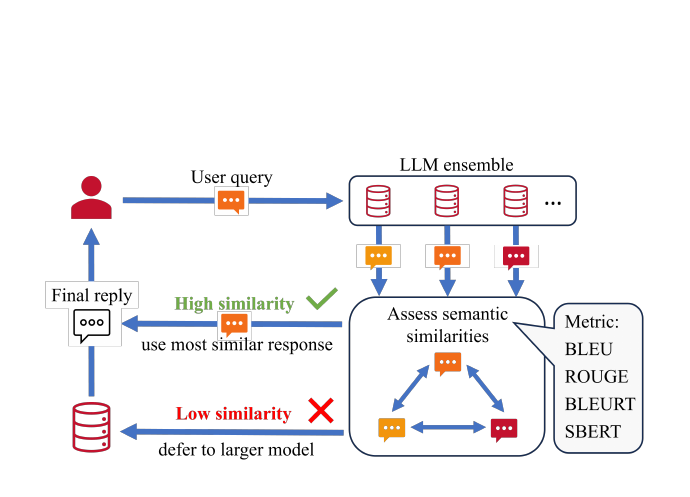
\includegraphics[width=2.676cm]{figures/img/method_gallery/tile_12.png}}};
\draw[black!35,line width=0.35pt] (5.562,-13.097) rectangle (8.238,-15.024);
\node[anchor=north west,text=ACMDarkBlue,font=\tiny\bfseries,inner sep=0] at (5.592,-15.054) {\href{https://arxiv.org/abs/2509.21837}{\adjustbox{max width=2.616cm}{Soiffer et al. 2025}}};
\node[anchor=north west,text=black!60,font=\tiny,inner sep=0] at (5.592,-15.259) {\href{https://arxiv.org/abs/2509.21837}{Fig. 1, p.~1}};
\node[anchor=north west,inner sep=0] at (8.308,-13.097) {\href{https://arxiv.org/abs/2305.11860}{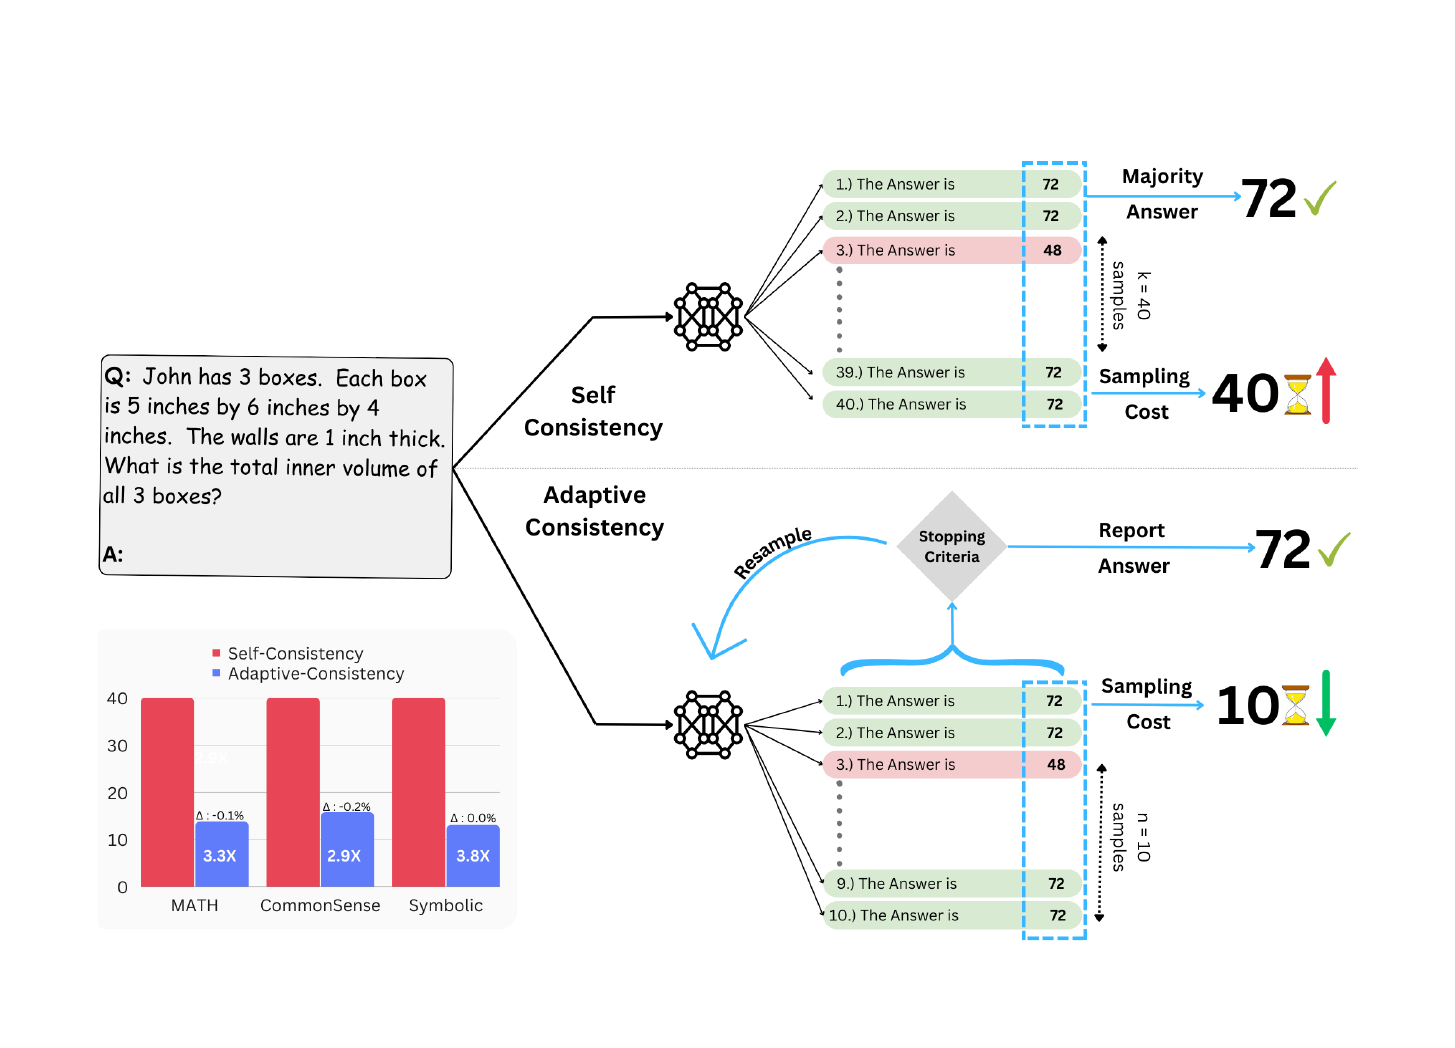
\includegraphics[width=2.676cm]{figures/img/method_gallery/tile_13.png}}};
\draw[black!35,line width=0.35pt] (8.308,-13.097) rectangle (10.984,-15.024);
\node[anchor=north west,text=ACMDarkBlue,font=\tiny\bfseries,inner sep=0] at (8.338,-15.054) {\href{https://arxiv.org/abs/2305.11860}{\adjustbox{max width=2.616cm}{Aggarwal et al. 2023}}};
\node[anchor=north west,text=black!60,font=\tiny,inner sep=0] at (8.338,-15.259) {\href{https://arxiv.org/abs/2305.11860}{Fig. 1, p.~2}};
\end{tikzpicture}}
\caption{\textbf{How confidence is produced and used, by stage.} Each panel shows a whole figure of the cited paper, reproduced under its CC BY licence; its label links to the paper. The selection rule and each panel's figure, page and licence are in Table~\ref{tab:panel_provenance}. S0 read-off has no panel: no reusable figure passed the check (Table~\ref{tab:panel_provenance}).}
\Description{A labelled grid of images, each a hyperlink annotated with its system name and source figure number.}
\label{fig:method_gallery}
\end{figure*}

% AUTO-GENERATED by build/gallery.py compile (pipeline tool gen_compilation_figure.py --fit)
% AUTO-GENERATED by tools/gen_compilation_figure.py -- vector TikZ, main-body, hyperlinked.
\begin{figure*}[tp]
\centering
\resizebox{\textwidth}{!}{%
\begin{tikzpicture}[x=1cm,y=1cm]
\definecolor{c626262}{HTML}{626262}
\definecolor{c355475}{HTML}{355475}
\definecolor{cAB5D10}{HTML}{AB5D10}
\definecolor{c3A7134}{HTML}{3A7134}
\definecolor{c7C5471}{HTML}{7C5471}
\definecolor{c9F3C3C}{HTML}{9F3C3C}
\fill[black!88] (0,0) rectangle (13.800,-0.580);
\node[anchor=west,text=white,font=\small\bfseries,inner sep=0] at (0.14,-0.290) {What calibration looks like in results, by stage};
\fill[c626262] (0,-0.580) rectangle (13.800,-1.080);
\node[anchor=west,text=white,font=\footnotesize\bfseries,inner sep=0] at (0.14,-0.830) {S0 read-off};
\node[anchor=north west,inner sep=0] at (4.189,-1.150) {\href{https://arxiv.org/abs/2211.07443}{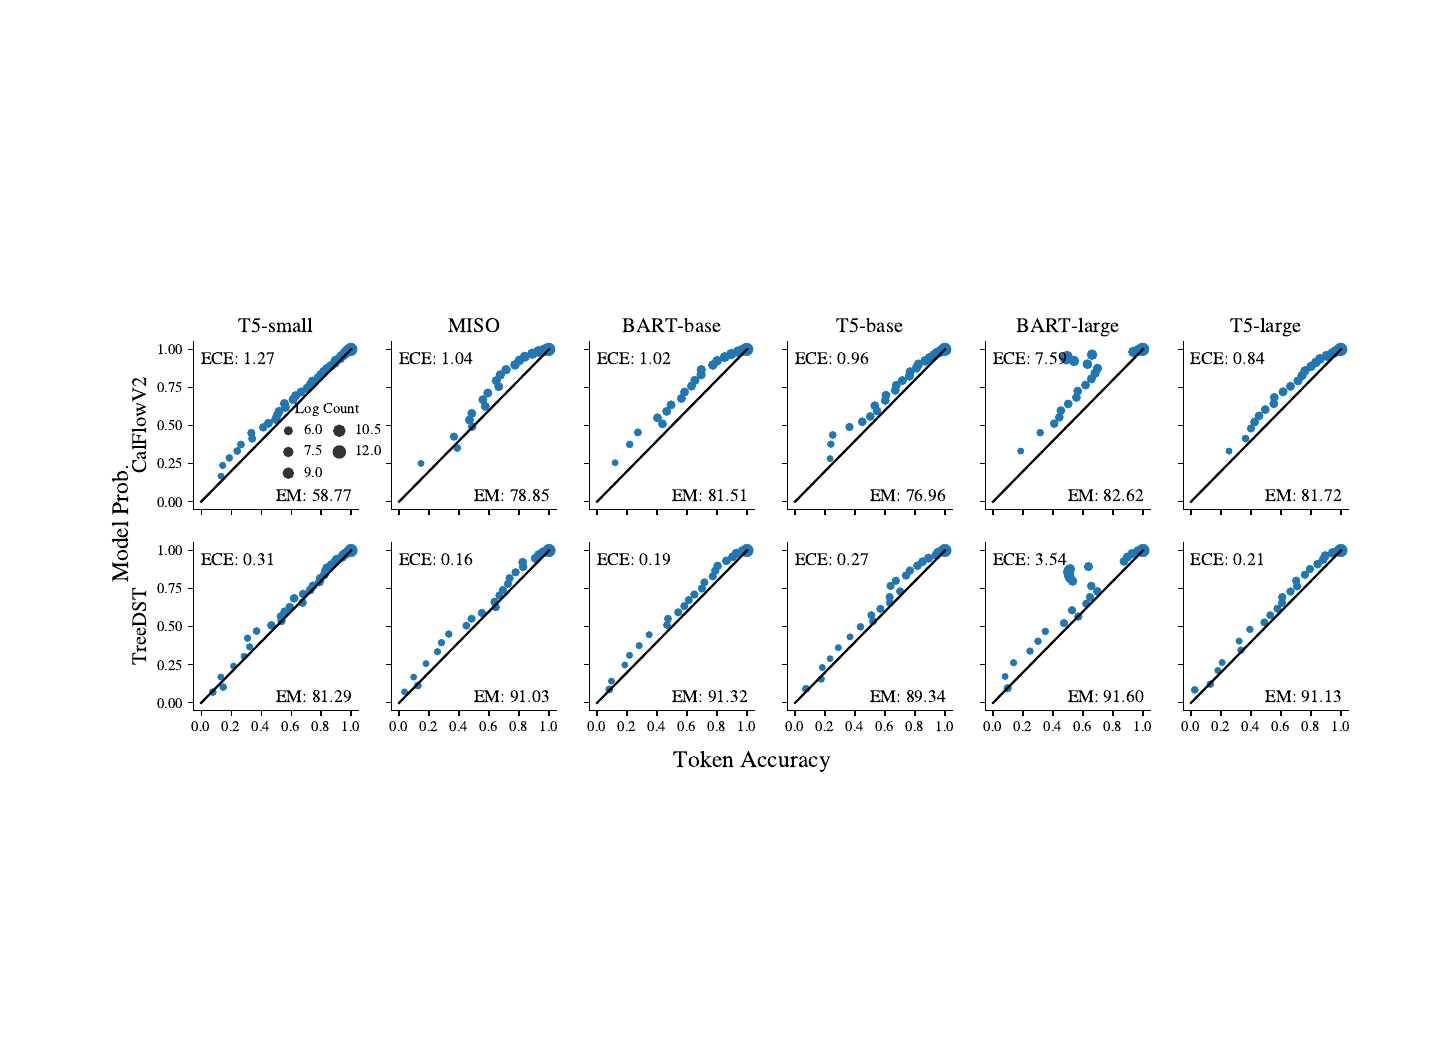
\includegraphics[width=2.676cm]{figures/img/results_gallery/tile_0.png}}};
\draw[black!35,line width=0.35pt] (4.189,-1.150) rectangle (6.865,-3.077);
\node[anchor=north west,text=ACMDarkBlue,font=\tiny\bfseries,inner sep=0] at (4.219,-3.107) {\href{https://arxiv.org/abs/2211.07443}{\adjustbox{max width=2.616cm}{Stengel-Eskin and Van Durme 2023}}};
\node[anchor=north west,text=black!60,font=\tiny,inner sep=0] at (4.219,-3.312) {\href{https://arxiv.org/abs/2211.07443}{Fig. 1, p.~6}};
\node[anchor=north west,inner sep=0] at (6.935,-1.150) {\href{https://arxiv.org/abs/2606.03437}{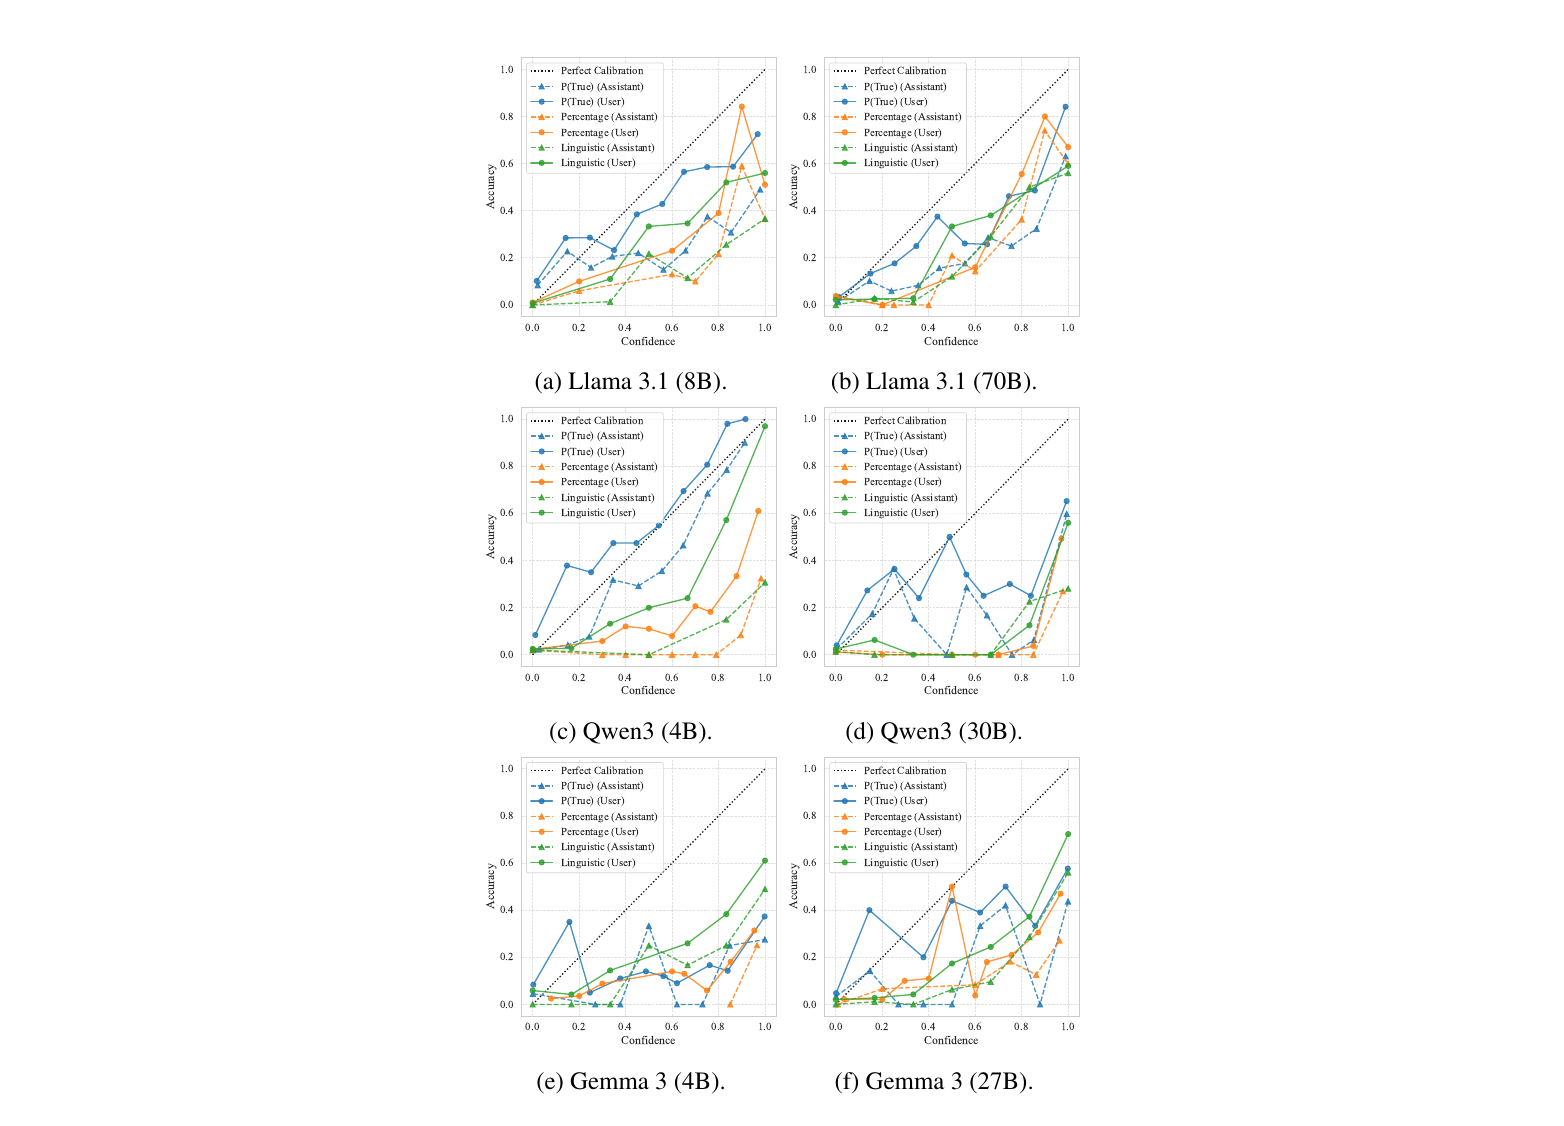
\includegraphics[width=2.676cm]{figures/img/results_gallery/tile_1.png}}};
\draw[black!35,line width=0.35pt] (6.935,-1.150) rectangle (9.611,-3.077);
\node[anchor=north west,text=ACMDarkBlue,font=\tiny\bfseries,inner sep=0] at (6.965,-3.107) {\href{https://arxiv.org/abs/2606.03437}{\adjustbox{max width=2.616cm}{Sanz-Guerrero et al. 2026}}};
\node[anchor=north west,text=black!60,font=\tiny,inner sep=0] at (6.965,-3.312) {\href{https://arxiv.org/abs/2606.03437}{Fig. 4, p.~6}};
\fill[c355475] (0,-3.567) rectangle (13.800,-4.067);
\node[anchor=west,text=white,font=\footnotesize\bfseries,inner sep=0] at (0.14,-3.817) {S1 post-hoc map};
\node[anchor=north west,inner sep=0] at (2.816,-4.137) {\href{https://arxiv.org/abs/2312.03729}{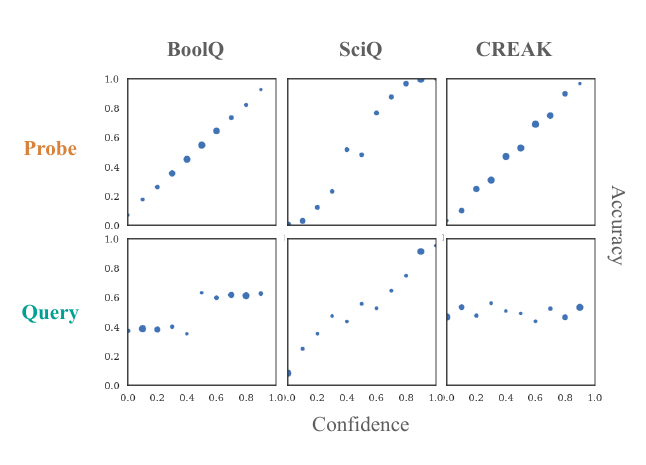
\includegraphics[width=2.676cm]{figures/img/results_gallery/tile_2.png}}};
\draw[black!35,line width=0.35pt] (2.816,-4.137) rectangle (5.492,-6.063);
\node[anchor=north west,text=ACMDarkBlue,font=\tiny\bfseries,inner sep=0] at (2.846,-6.093) {\href{https://arxiv.org/abs/2312.03729}{\adjustbox{max width=2.616cm}{Liu et al. 2023a}}};
\node[anchor=north west,text=black!60,font=\tiny,inner sep=0] at (2.846,-6.298) {\href{https://arxiv.org/abs/2312.03729}{Fig. 2, p.~3}};
\node[anchor=north west,inner sep=0] at (5.562,-4.137) {\href{https://arxiv.org/abs/2601.04277}{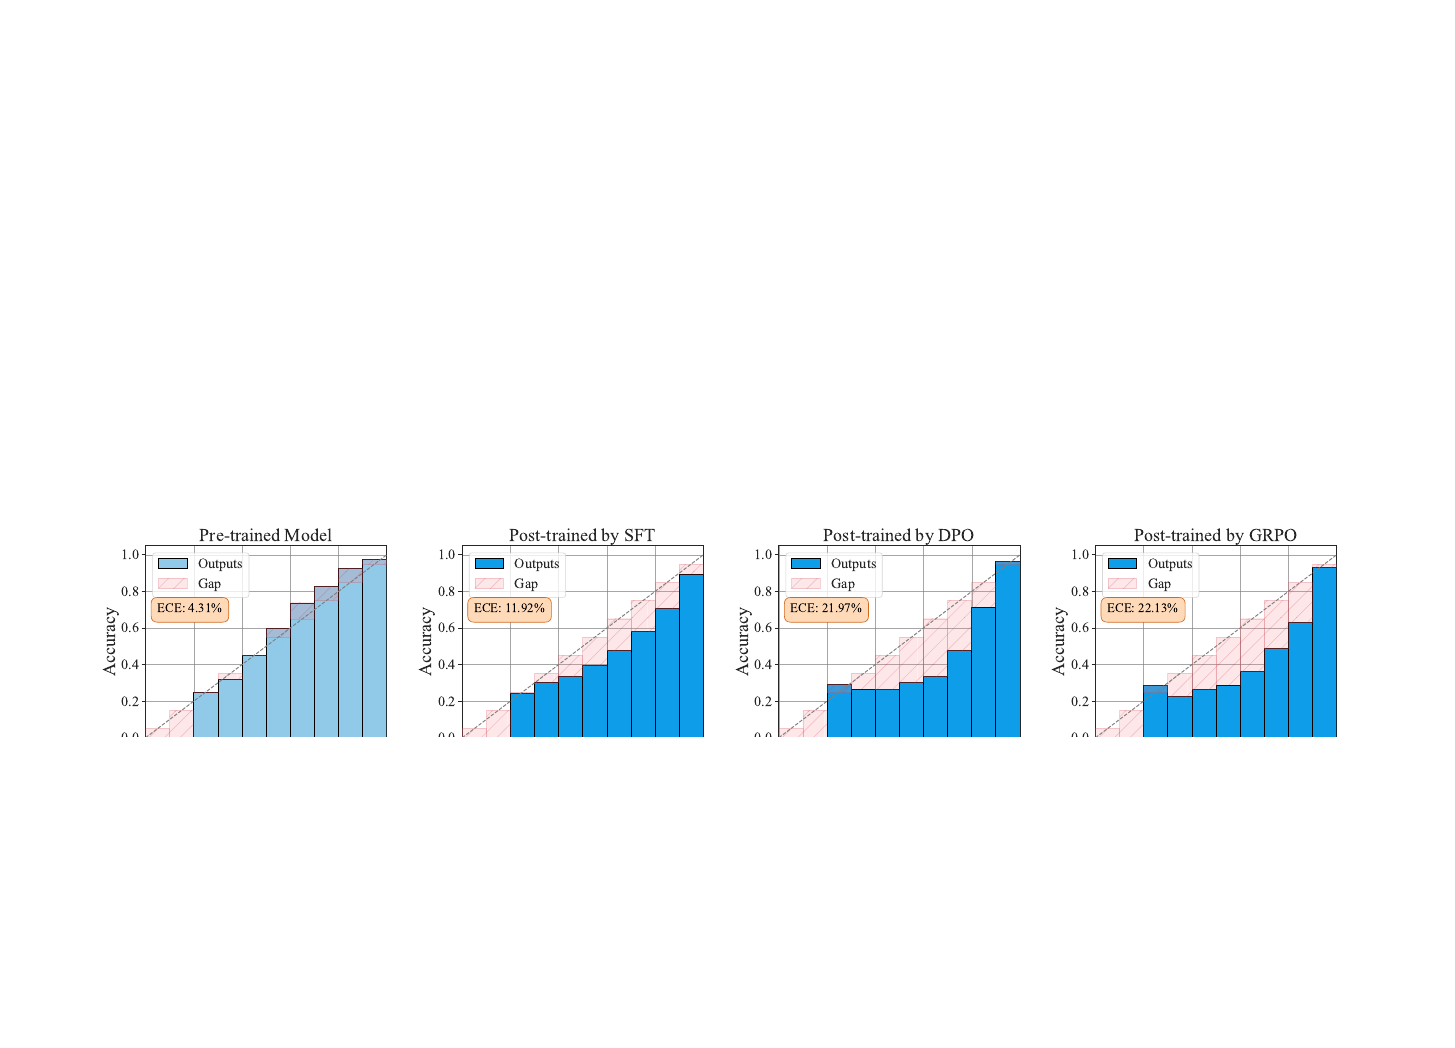
\includegraphics[width=2.676cm]{figures/img/results_gallery/tile_3.png}}};
\draw[black!35,line width=0.35pt] (5.562,-4.137) rectangle (8.238,-6.063);
\node[anchor=north west,text=ACMDarkBlue,font=\tiny\bfseries,inner sep=0] at (5.592,-6.093) {\href{https://arxiv.org/abs/2601.04277}{\adjustbox{max width=2.616cm}{Luo et al. 2026}}};
\node[anchor=north west,text=black!60,font=\tiny,inner sep=0] at (5.592,-6.298) {\href{https://arxiv.org/abs/2601.04277}{Fig. 5, p.~15}};
\node[anchor=north west,inner sep=0] at (8.308,-4.137) {\href{https://arxiv.org/abs/2505.16690}{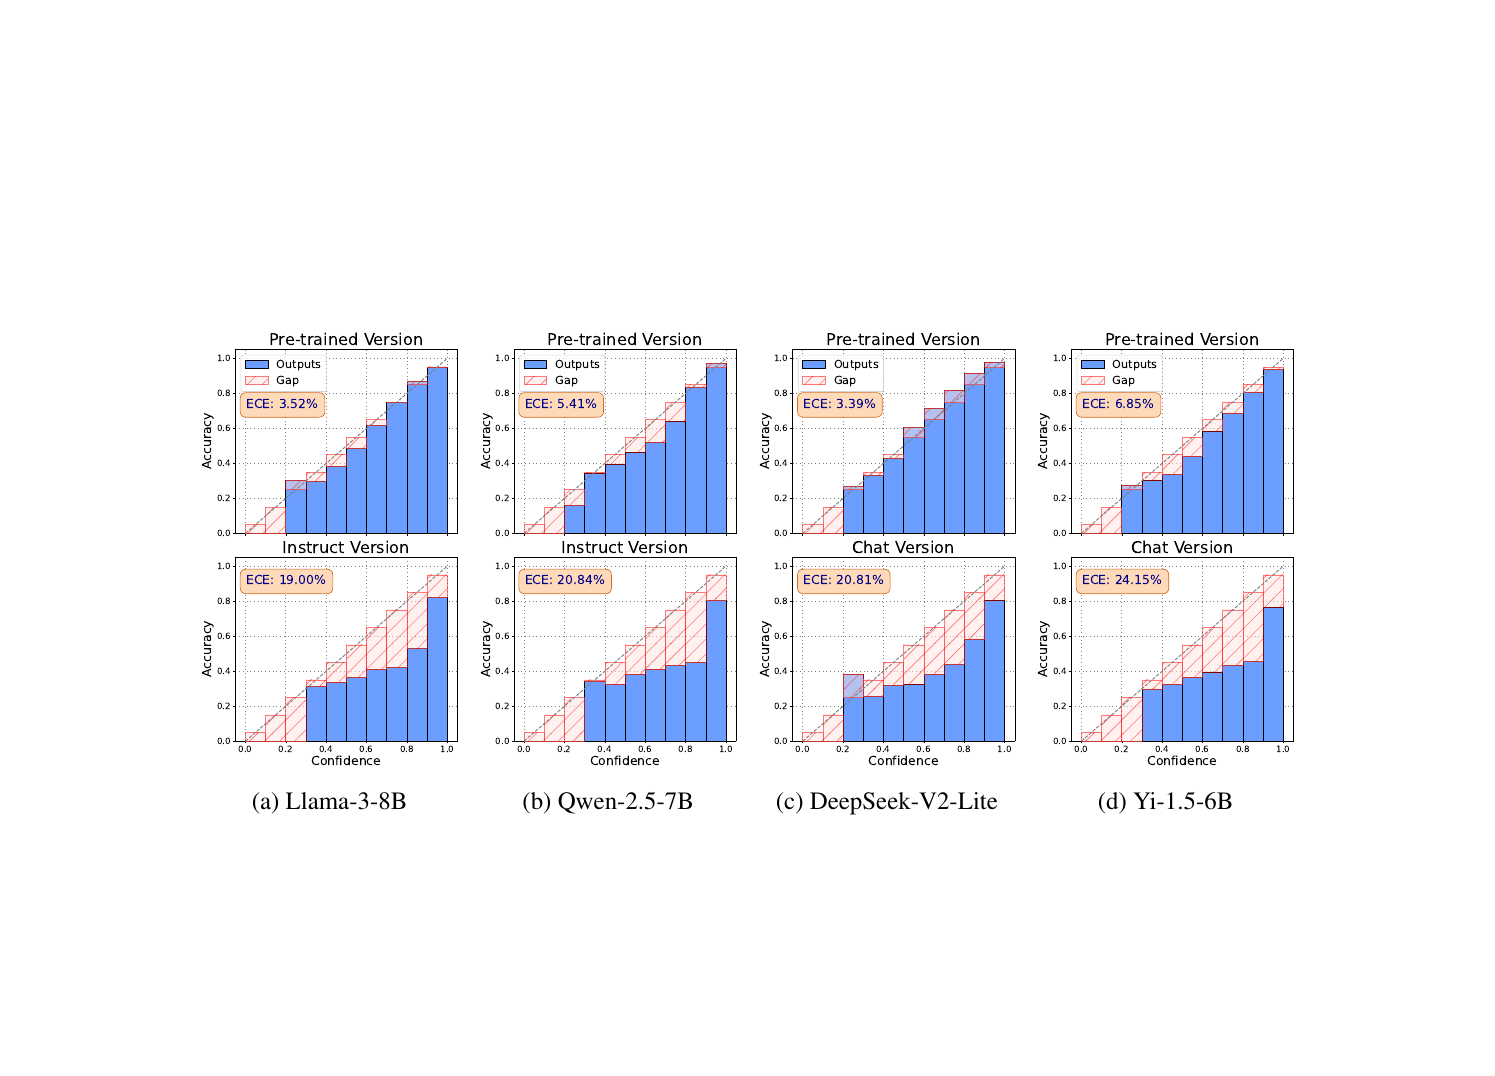
\includegraphics[width=2.676cm]{figures/img/results_gallery/tile_4.png}}};
\draw[black!35,line width=0.35pt] (8.308,-4.137) rectangle (10.984,-6.063);
\node[anchor=north west,text=ACMDarkBlue,font=\tiny\bfseries,inner sep=0] at (8.338,-6.093) {\href{https://arxiv.org/abs/2505.16690}{\adjustbox{max width=2.616cm}{Luo et al. 2025}}};
\node[anchor=north west,text=black!60,font=\tiny,inner sep=0] at (8.338,-6.298) {\href{https://arxiv.org/abs/2505.16690}{Fig. 1, p.~3}};
\fill[cAB5D10] (0,-6.553) rectangle (13.800,-7.053);
\node[anchor=west,text=white,font=\footnotesize\bfseries,inner sep=0] at (0.14,-6.803) {S2 prompt elicitation};
\node[anchor=north west,inner sep=0] at (2.816,-7.123) {\href{https://arxiv.org/abs/2606.17234}{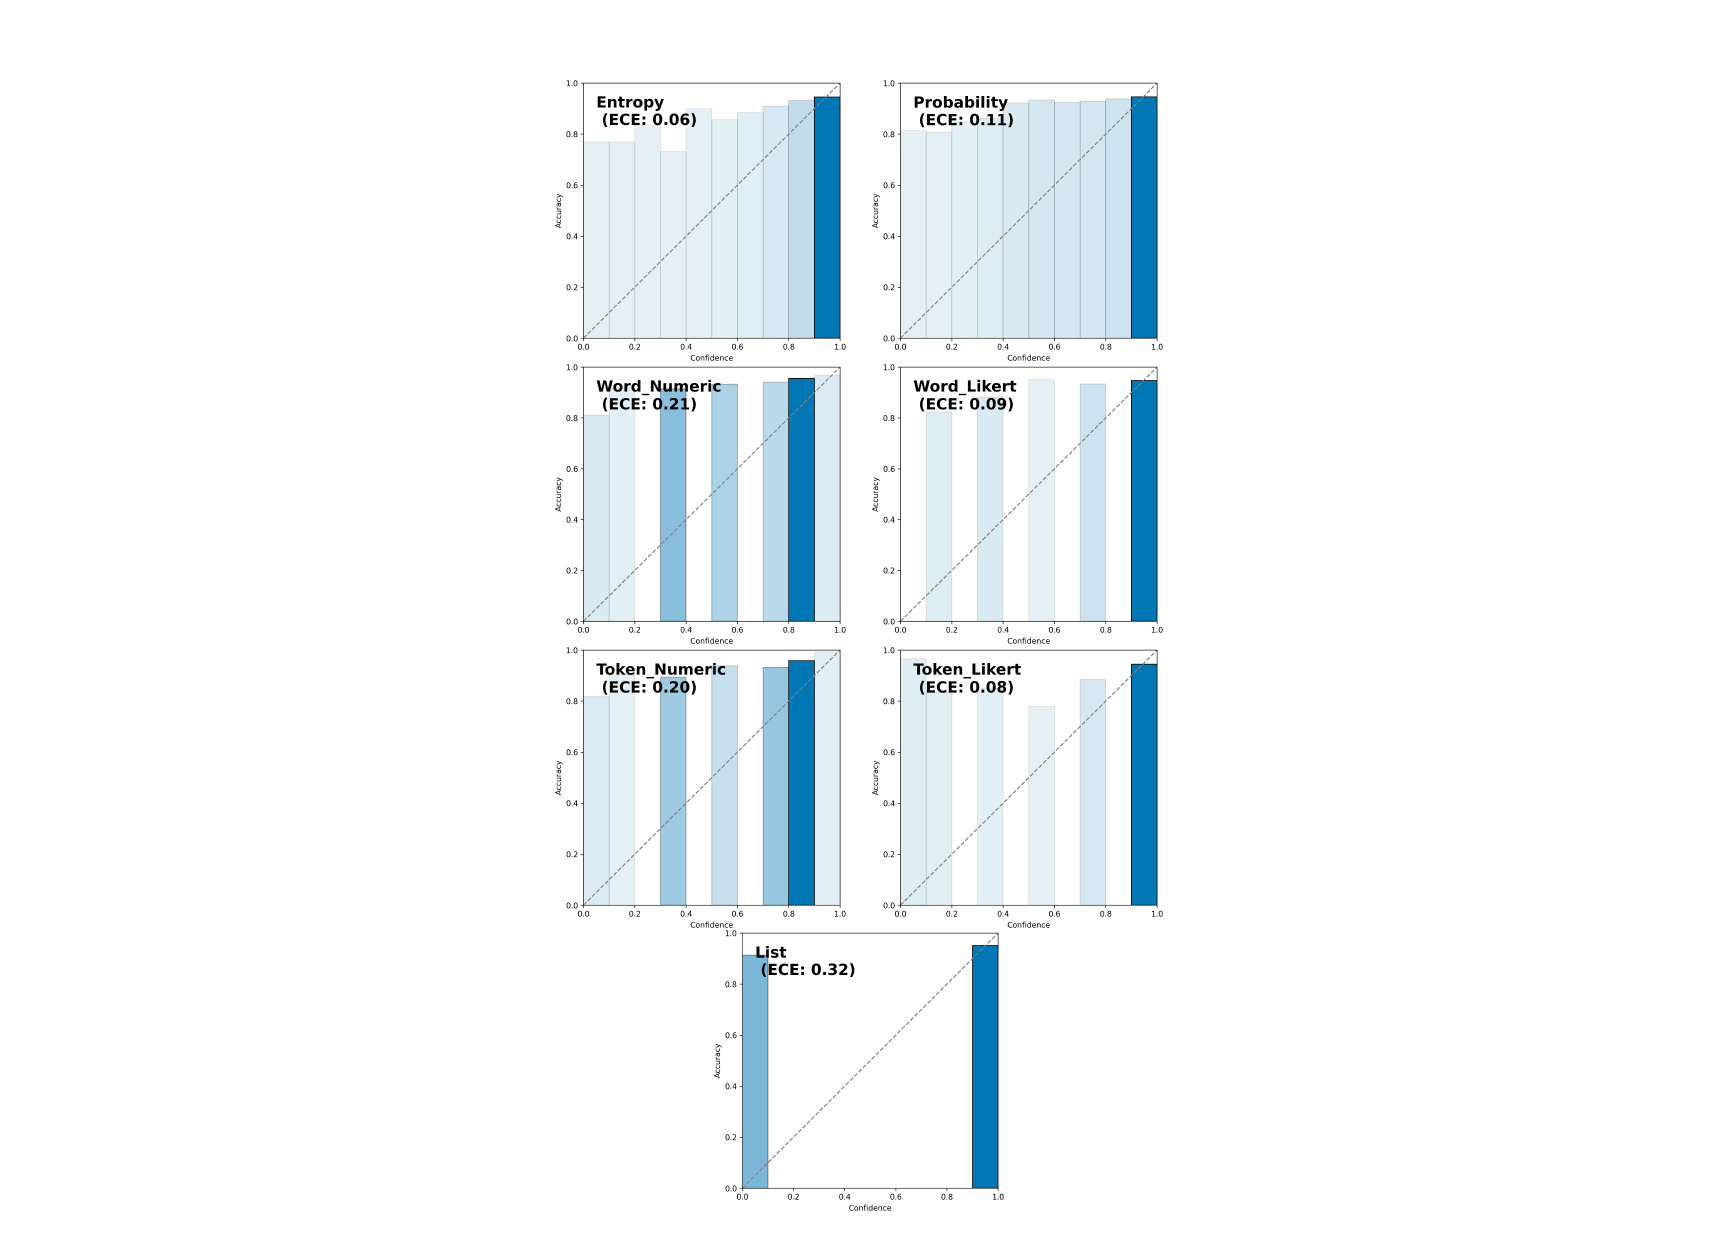
\includegraphics[width=2.676cm]{figures/img/results_gallery/tile_5.png}}};
\draw[black!35,line width=0.35pt] (2.816,-7.123) rectangle (5.492,-9.050);
\node[anchor=north west,text=ACMDarkBlue,font=\tiny\bfseries,inner sep=0] at (2.846,-9.080) {\href{https://arxiv.org/abs/2606.17234}{\adjustbox{max width=2.616cm}{Marashian et al. 2026}}};
\node[anchor=north west,text=black!60,font=\tiny,inner sep=0] at (2.846,-9.285) {\href{https://arxiv.org/abs/2606.17234}{Fig. 2, p.~5}};
\node[anchor=north west,inner sep=0] at (5.562,-7.123) {\href{https://arxiv.org/abs/2404.09127}{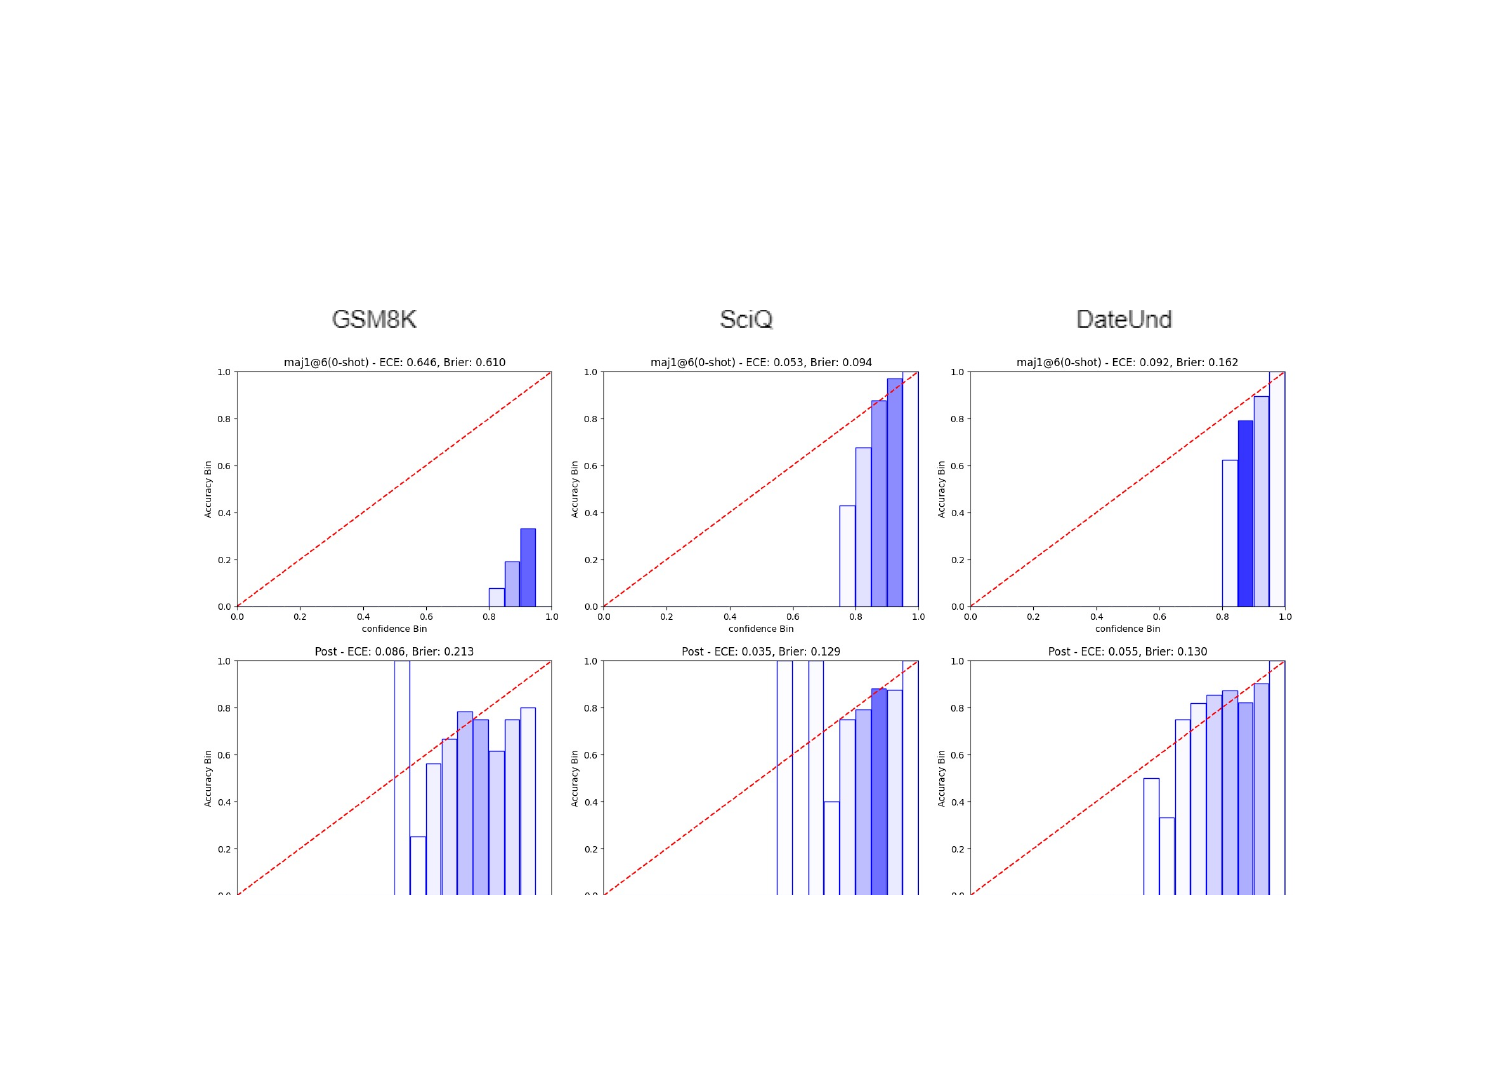
\includegraphics[width=2.676cm]{figures/img/results_gallery/tile_6.png}}};
\draw[black!35,line width=0.35pt] (5.562,-7.123) rectangle (8.238,-9.050);
\node[anchor=north west,text=ACMDarkBlue,font=\tiny\bfseries,inner sep=0] at (5.592,-9.080) {\href{https://arxiv.org/abs/2404.09127}{\adjustbox{max width=2.616cm}{Yang et al. 2024c}}};
\node[anchor=north west,text=black!60,font=\tiny,inner sep=0] at (5.592,-9.285) {\href{https://arxiv.org/abs/2404.09127}{Fig. 3, p.~11}};
\node[anchor=north west,inner sep=0] at (8.308,-7.123) {\href{https://arxiv.org/abs/2603.29559}{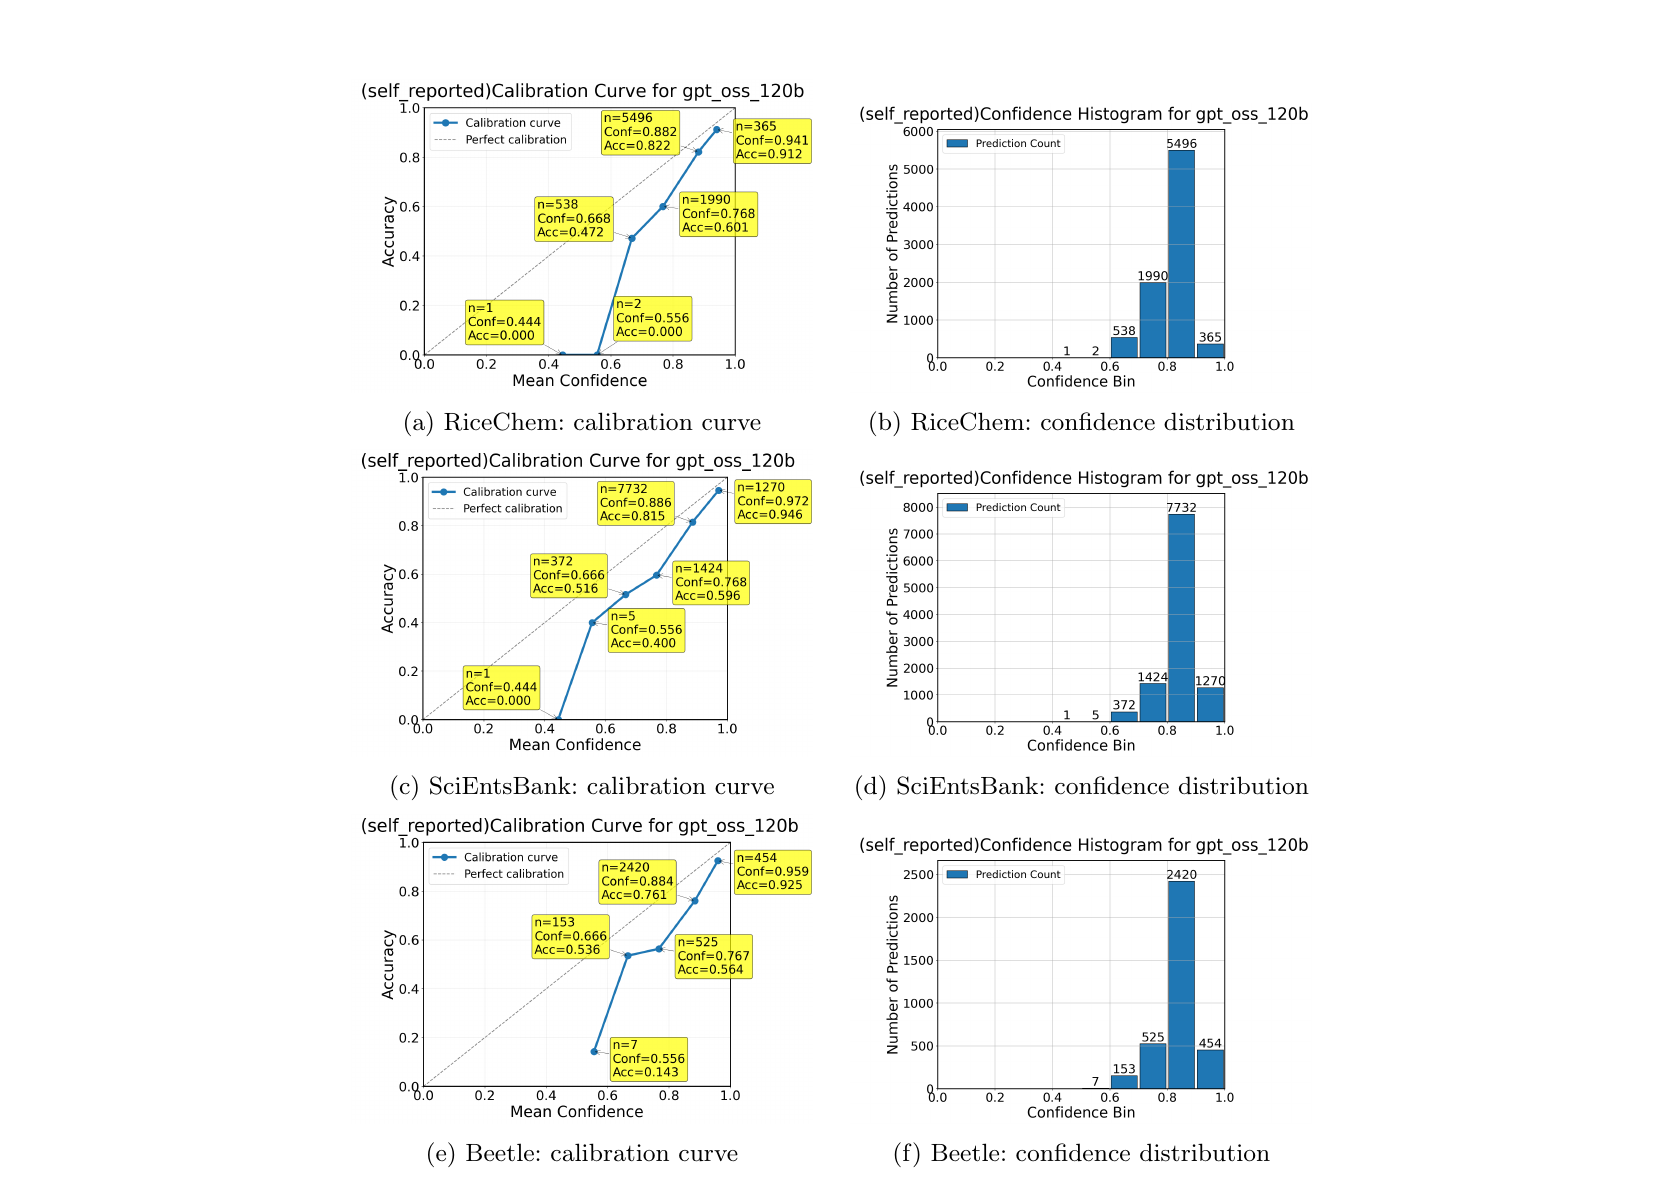
\includegraphics[width=2.676cm]{figures/img/results_gallery/tile_7.png}}};
\draw[black!35,line width=0.35pt] (8.308,-7.123) rectangle (10.984,-9.050);
\node[anchor=north west,text=ACMDarkBlue,font=\tiny\bfseries,inner sep=0] at (8.338,-9.080) {\href{https://arxiv.org/abs/2603.29559}{\adjustbox{max width=2.616cm}{Ferrer et al. 2026}}};
\node[anchor=north west,text=black!60,font=\tiny,inner sep=0] at (8.338,-9.285) {\href{https://arxiv.org/abs/2603.29559}{Fig. 1, p.~10}};
\fill[c3A7134] (0,-9.540) rectangle (13.800,-10.040);
\node[anchor=west,text=white,font=\footnotesize\bfseries,inner sep=0] at (0.14,-9.790) {S3 extra inference};
\node[anchor=north west,inner sep=0] at (2.816,-10.110) {\href{https://arxiv.org/abs/2402.00707}{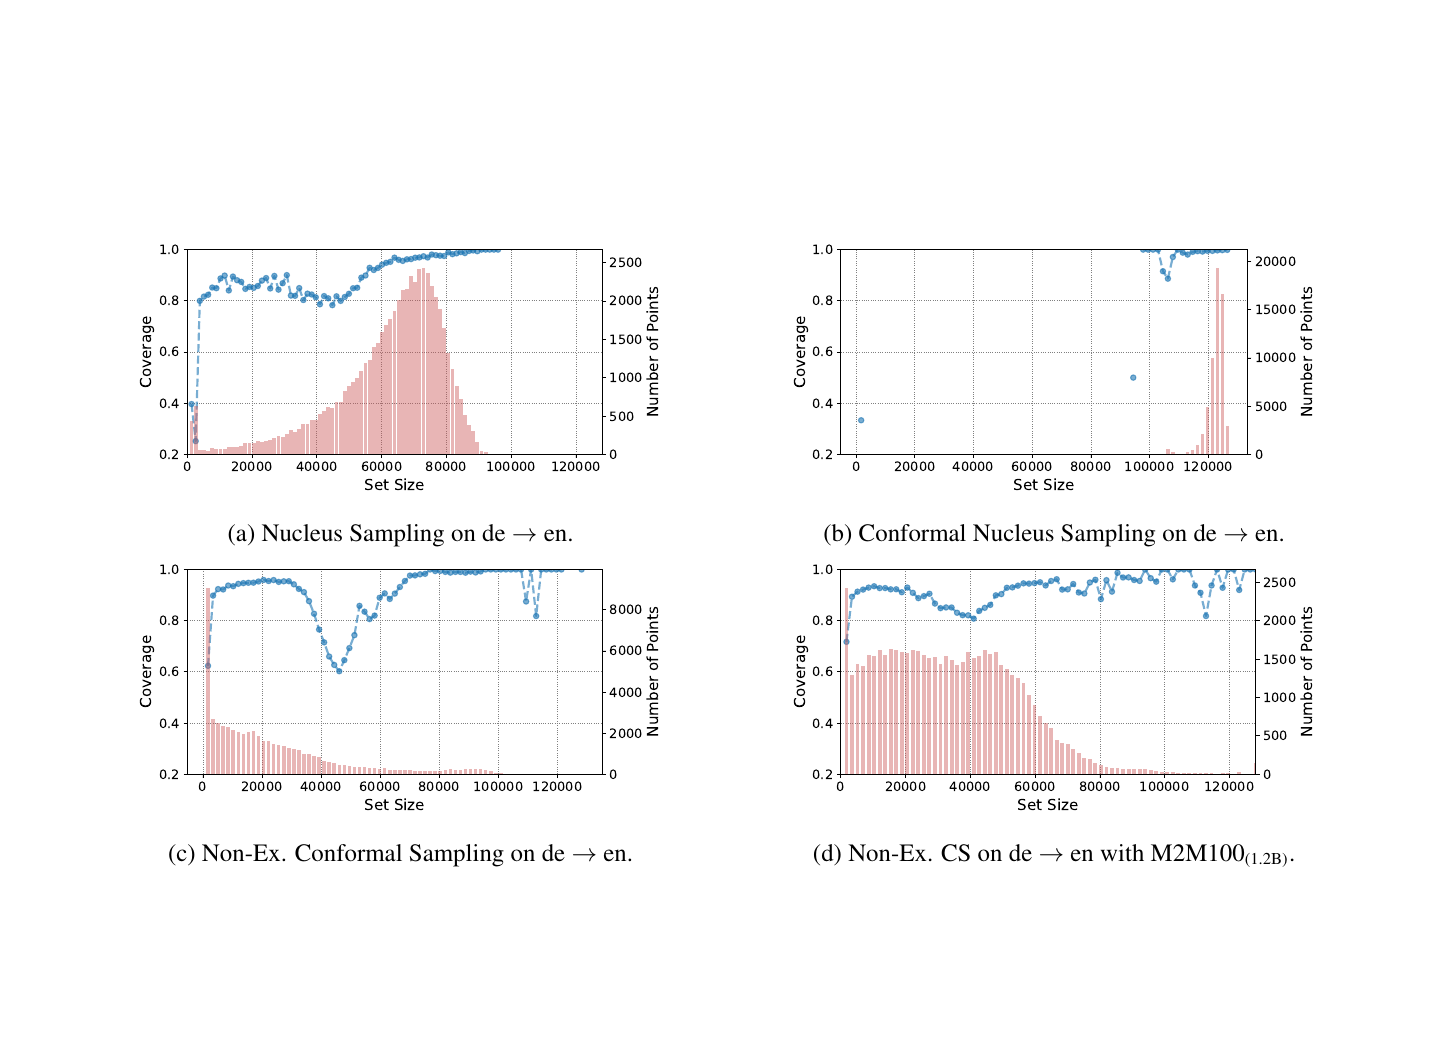
\includegraphics[width=2.676cm]{figures/img/results_gallery/tile_8.png}}};
\draw[black!35,line width=0.35pt] (2.816,-10.110) rectangle (5.492,-12.037);
\node[anchor=north west,text=ACMDarkBlue,font=\tiny\bfseries,inner sep=0] at (2.846,-12.067) {\href{https://arxiv.org/abs/2402.00707}{\adjustbox{max width=2.616cm}{Ulmer et al. 2024b}}};
\node[anchor=north west,text=black!60,font=\tiny,inner sep=0] at (2.846,-12.272) {\href{https://arxiv.org/abs/2402.00707}{Fig. 2, p.~6}};
\node[anchor=north west,inner sep=0] at (5.562,-10.110) {\href{https://arxiv.org/abs/2602.03814}{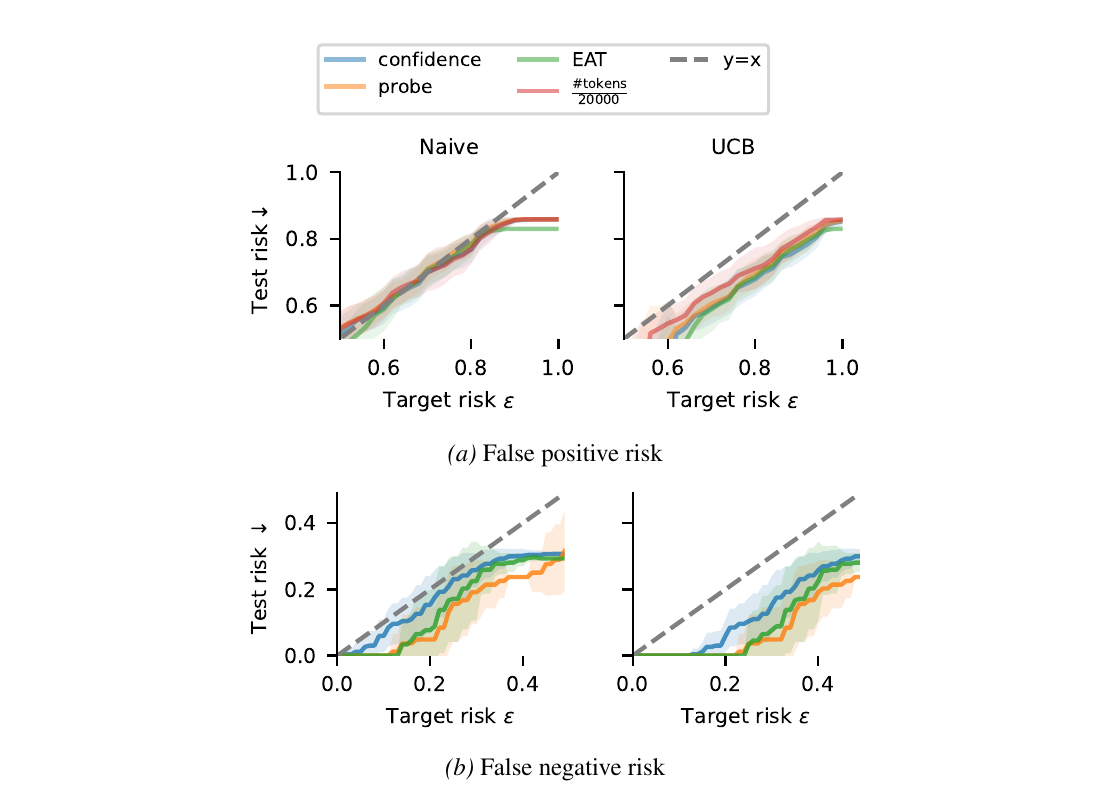
\includegraphics[width=2.676cm]{figures/img/results_gallery/tile_9.png}}};
\draw[black!35,line width=0.35pt] (5.562,-10.110) rectangle (8.238,-12.037);
\node[anchor=north west,text=ACMDarkBlue,font=\tiny\bfseries,inner sep=0] at (5.592,-12.067) {\href{https://arxiv.org/abs/2602.03814}{\adjustbox{max width=2.616cm}{Wang et al. 2026b}}};
\node[anchor=north west,text=black!60,font=\tiny,inner sep=0] at (5.592,-12.272) {\href{https://arxiv.org/abs/2602.03814}{Fig. 4, p.~7}};
\node[anchor=north west,inner sep=0] at (8.308,-10.110) {\href{https://arxiv.org/abs/2406.09714}{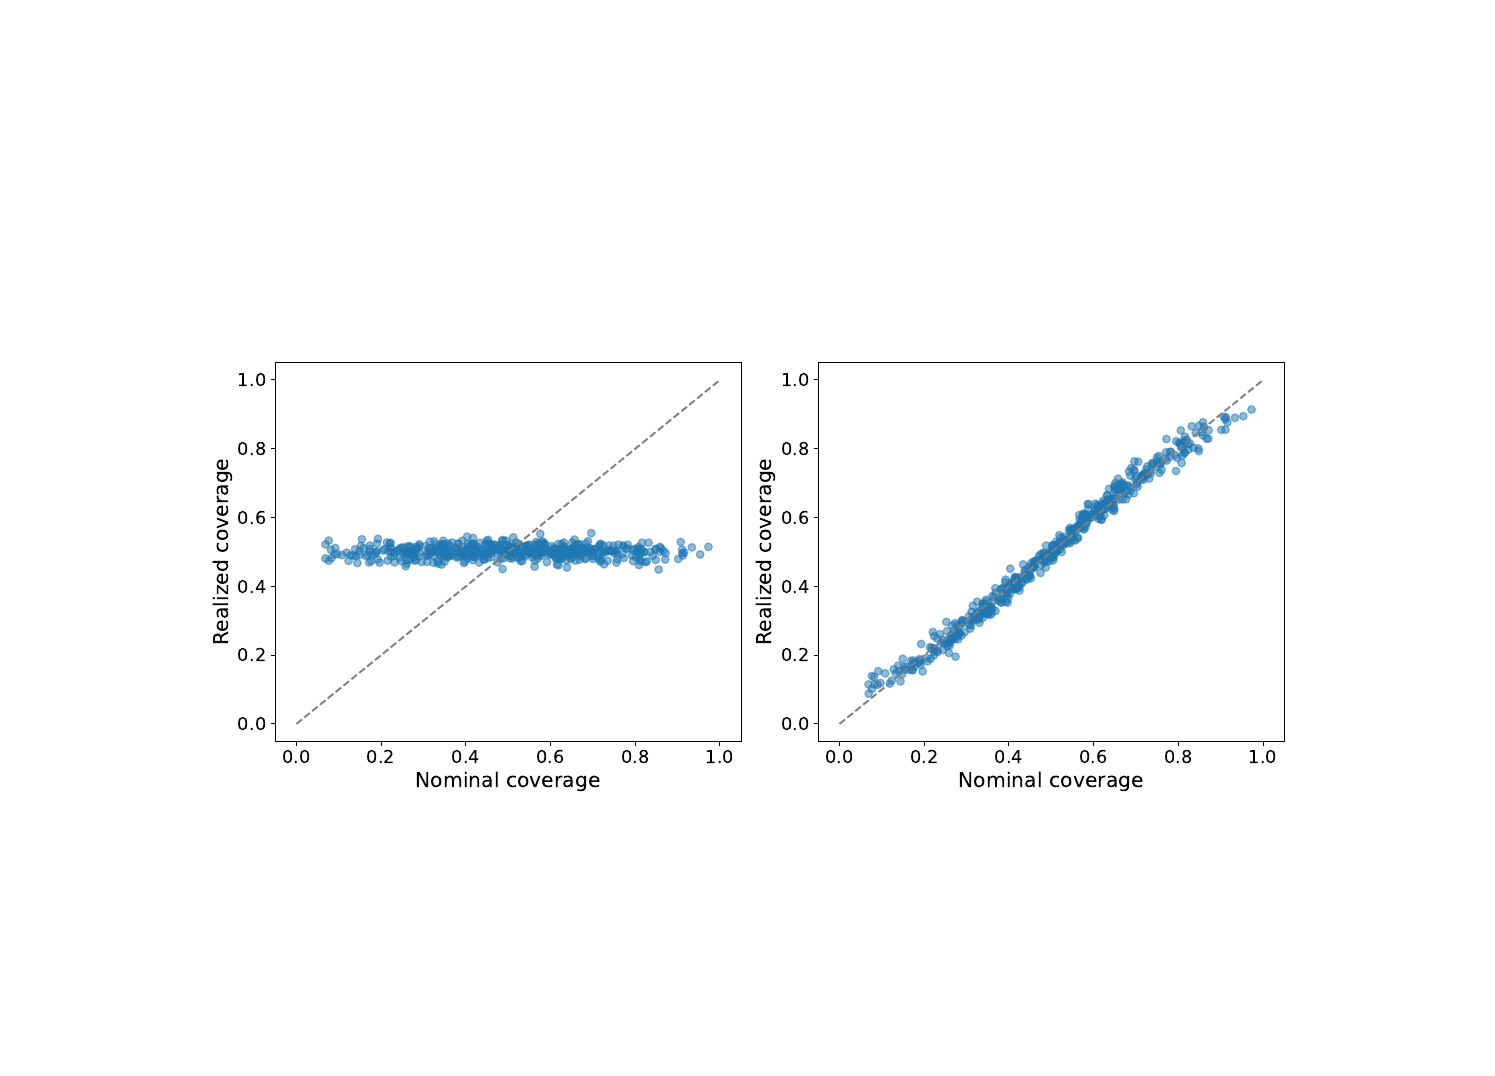
\includegraphics[width=2.676cm]{figures/img/results_gallery/tile_10.png}}};
\draw[black!35,line width=0.35pt] (8.308,-10.110) rectangle (10.984,-12.037);
\node[anchor=north west,text=ACMDarkBlue,font=\tiny\bfseries,inner sep=0] at (8.338,-12.067) {\href{https://arxiv.org/abs/2406.09714}{\adjustbox{max width=2.616cm}{Cherian et al. 2024}}};
\node[anchor=north west,text=black!60,font=\tiny,inner sep=0] at (8.338,-12.272) {\href{https://arxiv.org/abs/2406.09714}{Fig. 8, p.~18}};
\fill[c7C5471] (0,-12.527) rectangle (13.800,-13.027);
\node[anchor=west,text=white,font=\footnotesize\bfseries,inner sep=0] at (0.14,-12.777) {S4 training};
\node[anchor=north west,inner sep=0] at (4.189,-13.097) {\href{https://arxiv.org/abs/2607.04332}{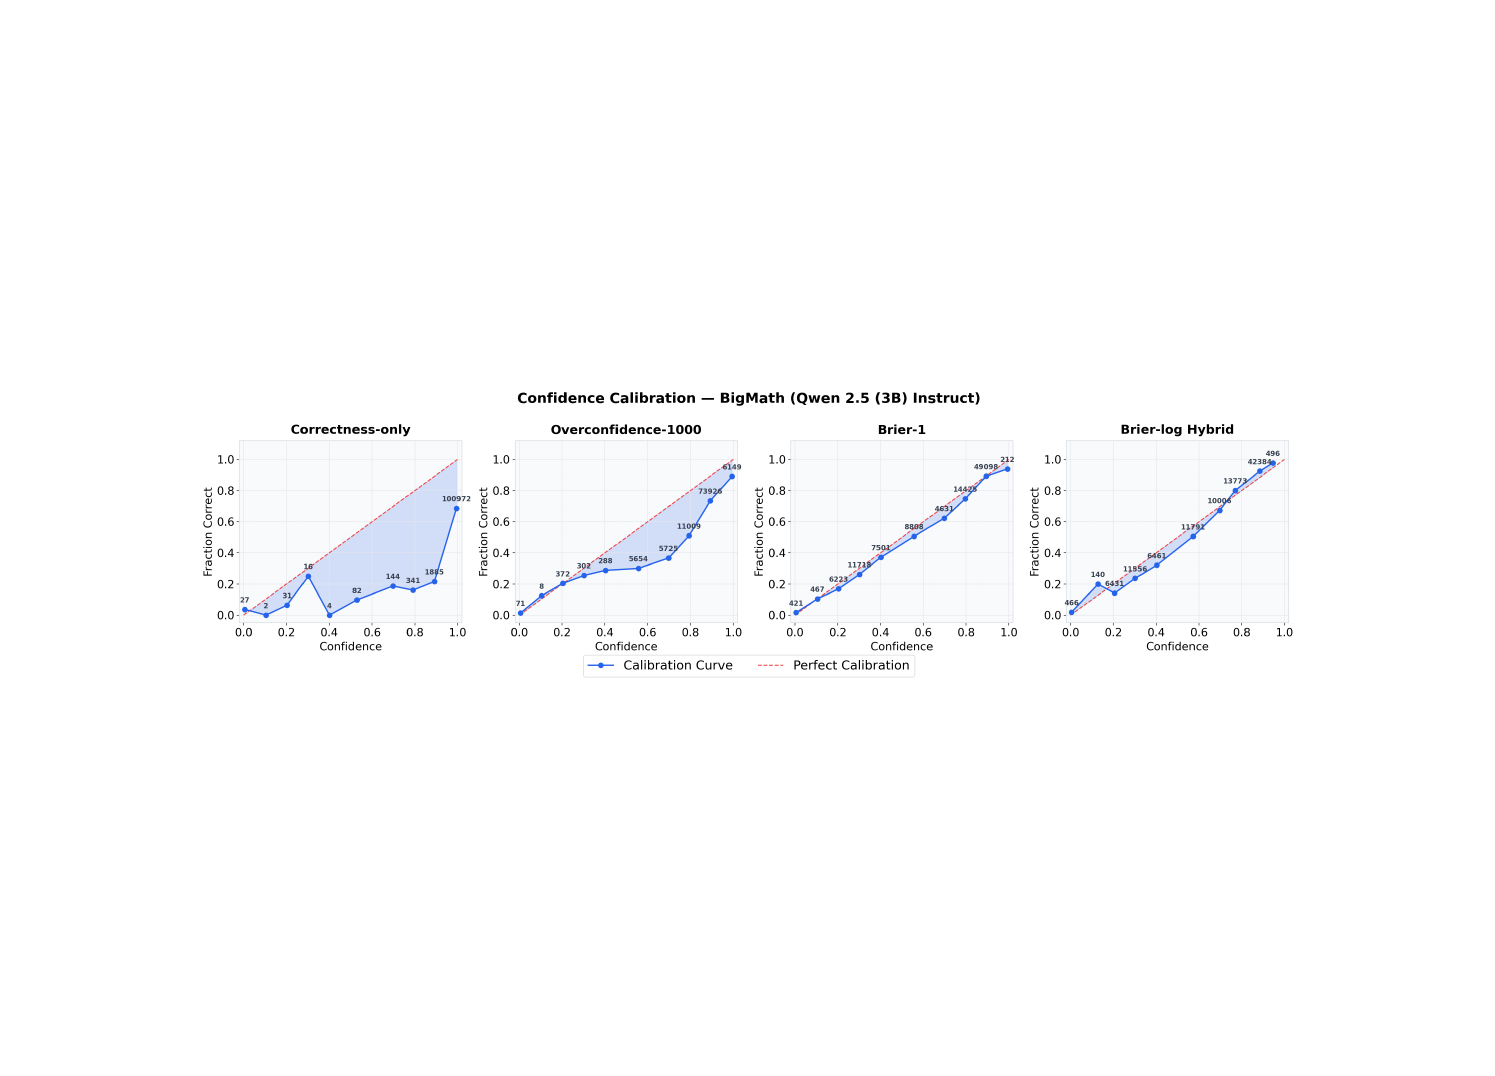
\includegraphics[width=2.676cm]{figures/img/results_gallery/tile_11.png}}};
\draw[black!35,line width=0.35pt] (4.189,-13.097) rectangle (6.865,-15.024);
\node[anchor=north west,text=ACMDarkBlue,font=\tiny\bfseries,inner sep=0] at (4.219,-15.054) {\href{https://arxiv.org/abs/2607.04332}{\adjustbox{max width=2.616cm}{Tan et al. 2026}}};
\node[anchor=north west,text=black!60,font=\tiny,inner sep=0] at (4.219,-15.259) {\href{https://arxiv.org/abs/2607.04332}{Fig. 4, p.~8}};
\node[anchor=north west,inner sep=0] at (6.935,-13.097) {\href{https://arxiv.org/abs/2510.05126}{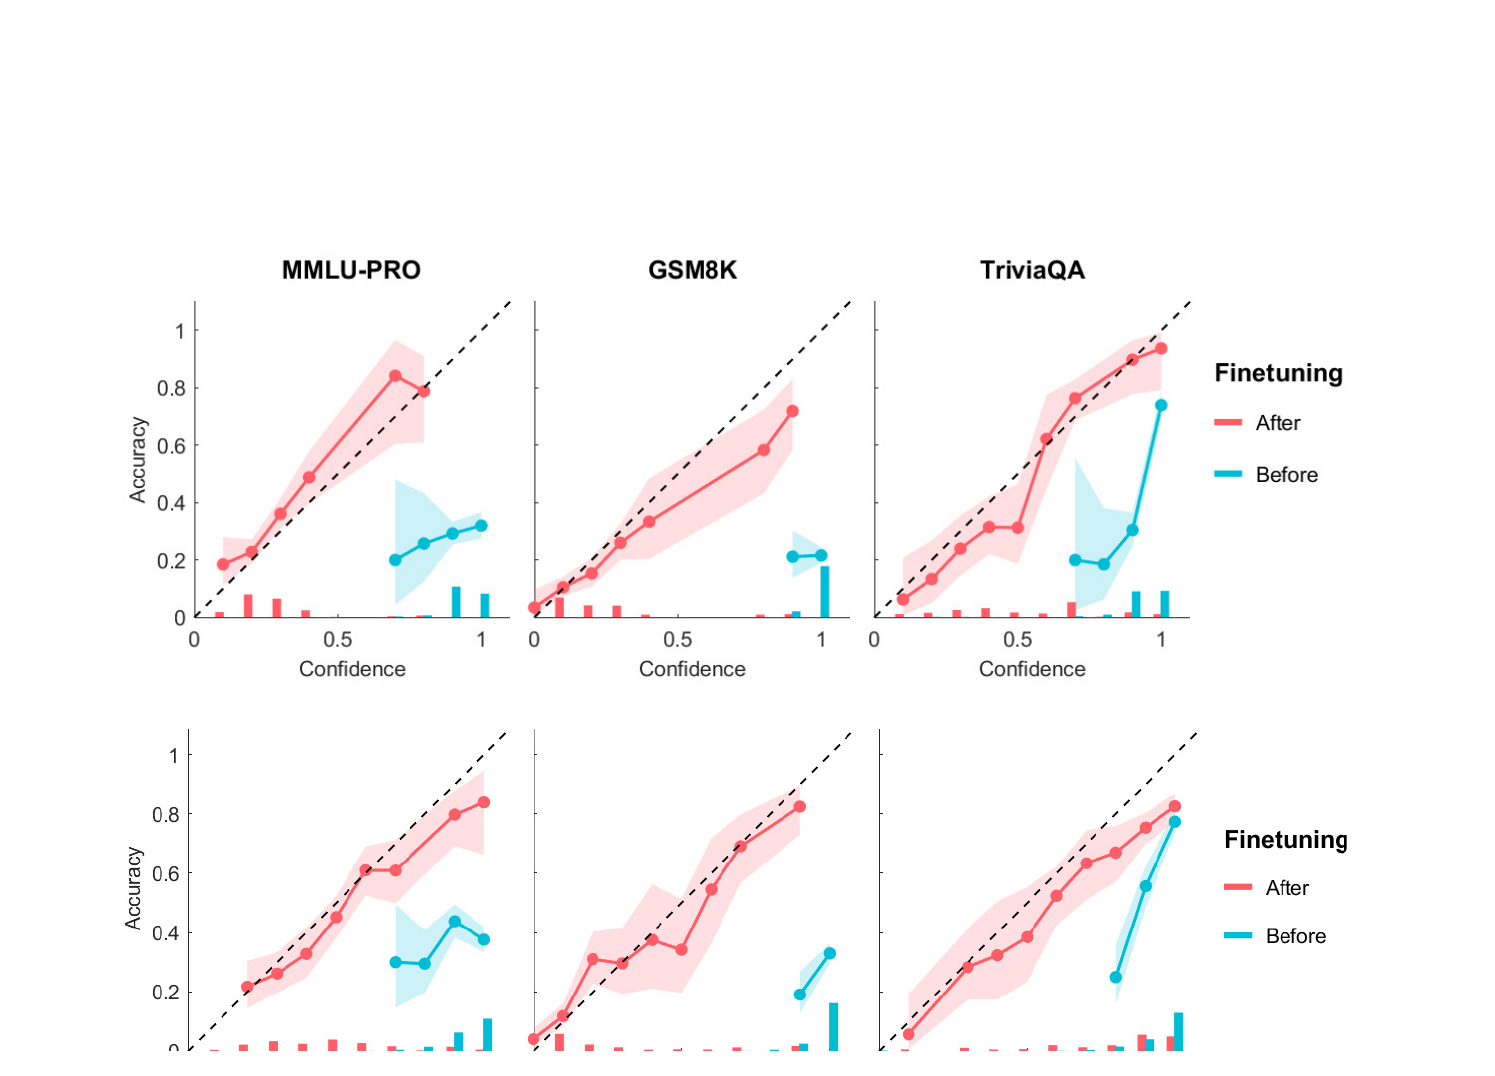
\includegraphics[width=2.676cm]{figures/img/results_gallery/tile_12.png}}};
\draw[black!35,line width=0.35pt] (6.935,-13.097) rectangle (9.611,-15.024);
\node[anchor=north west,text=ACMDarkBlue,font=\tiny\bfseries,inner sep=0] at (6.965,-15.054) {\href{https://arxiv.org/abs/2510.05126}{\adjustbox{max width=2.616cm}{Steyvers et al. 2025a}}};
\node[anchor=north west,text=black!60,font=\tiny,inner sep=0] at (6.965,-15.259) {\href{https://arxiv.org/abs/2510.05126}{Fig. 3, p.~7}};
\fill[c9F3C3C] (0,-15.514) rectangle (13.800,-16.014);
\node[anchor=west,text=white,font=\footnotesize\bfseries,inner sep=0] at (0.14,-15.764) {X consumers and contract};
\node[anchor=north west,inner sep=0] at (2.816,-16.084) {\href{https://arxiv.org/abs/2509.21837}{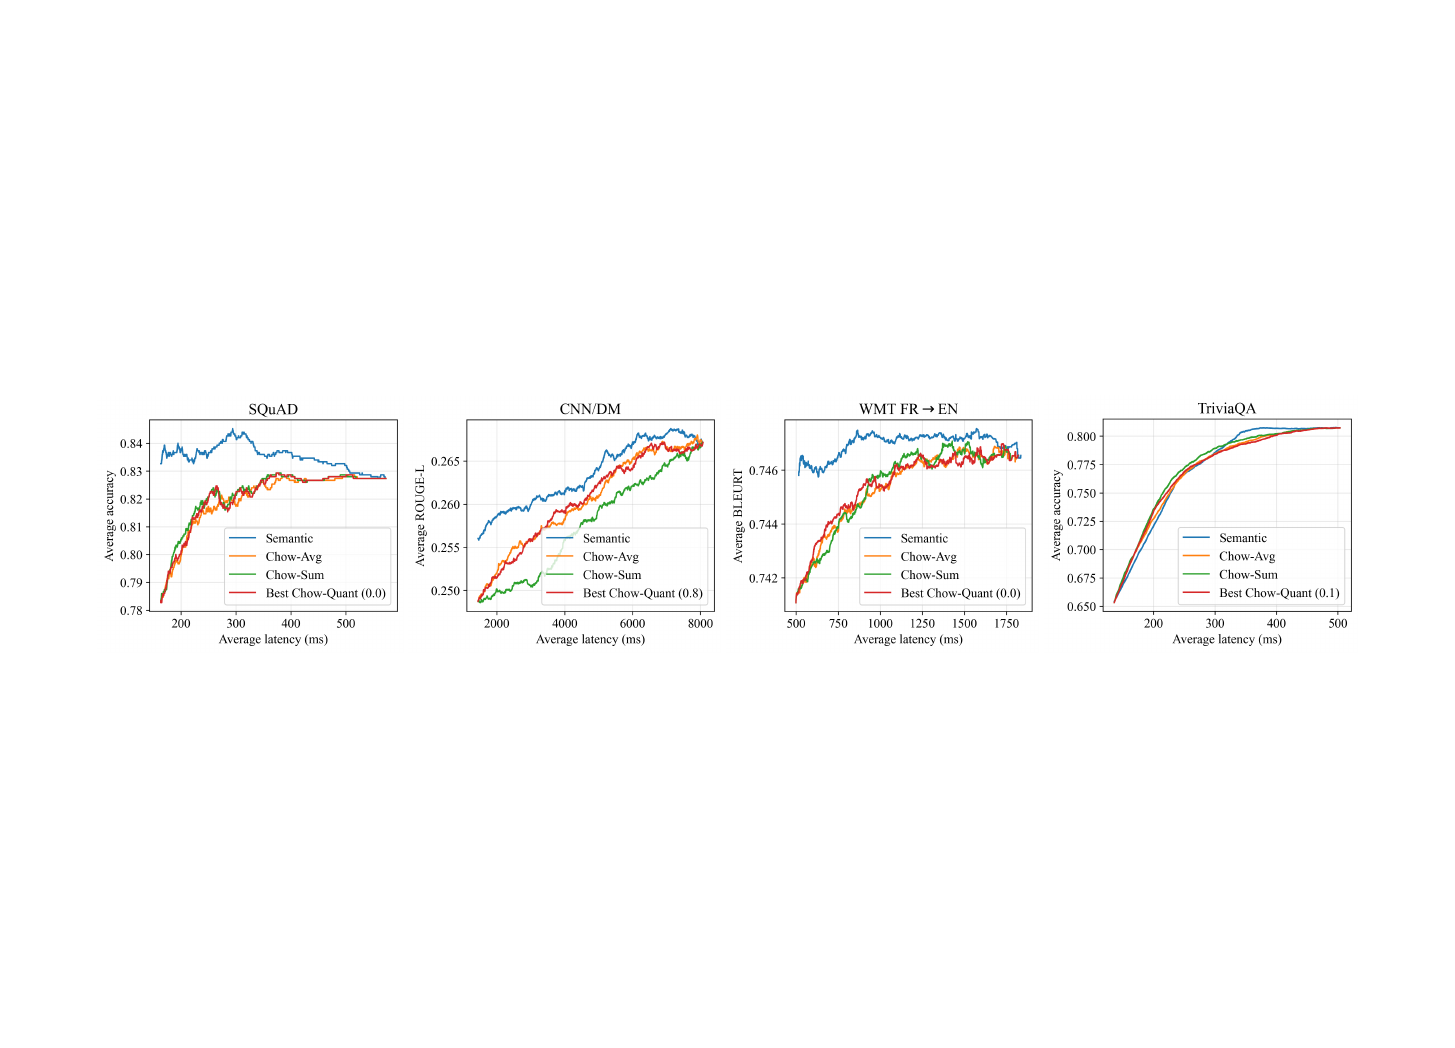
\includegraphics[width=2.676cm]{figures/img/results_gallery/tile_13.png}}};
\draw[black!35,line width=0.35pt] (2.816,-16.084) rectangle (5.492,-18.010);
\node[anchor=north west,text=ACMDarkBlue,font=\tiny\bfseries,inner sep=0] at (2.846,-18.040) {\href{https://arxiv.org/abs/2509.21837}{\adjustbox{max width=2.616cm}{Soiffer et al. 2025}}};
\node[anchor=north west,text=black!60,font=\tiny,inner sep=0] at (2.846,-18.245) {\href{https://arxiv.org/abs/2509.21837}{Fig. 2, p.~5}};
\node[anchor=north west,inner sep=0] at (5.562,-16.084) {\href{https://arxiv.org/abs/2506.11887}{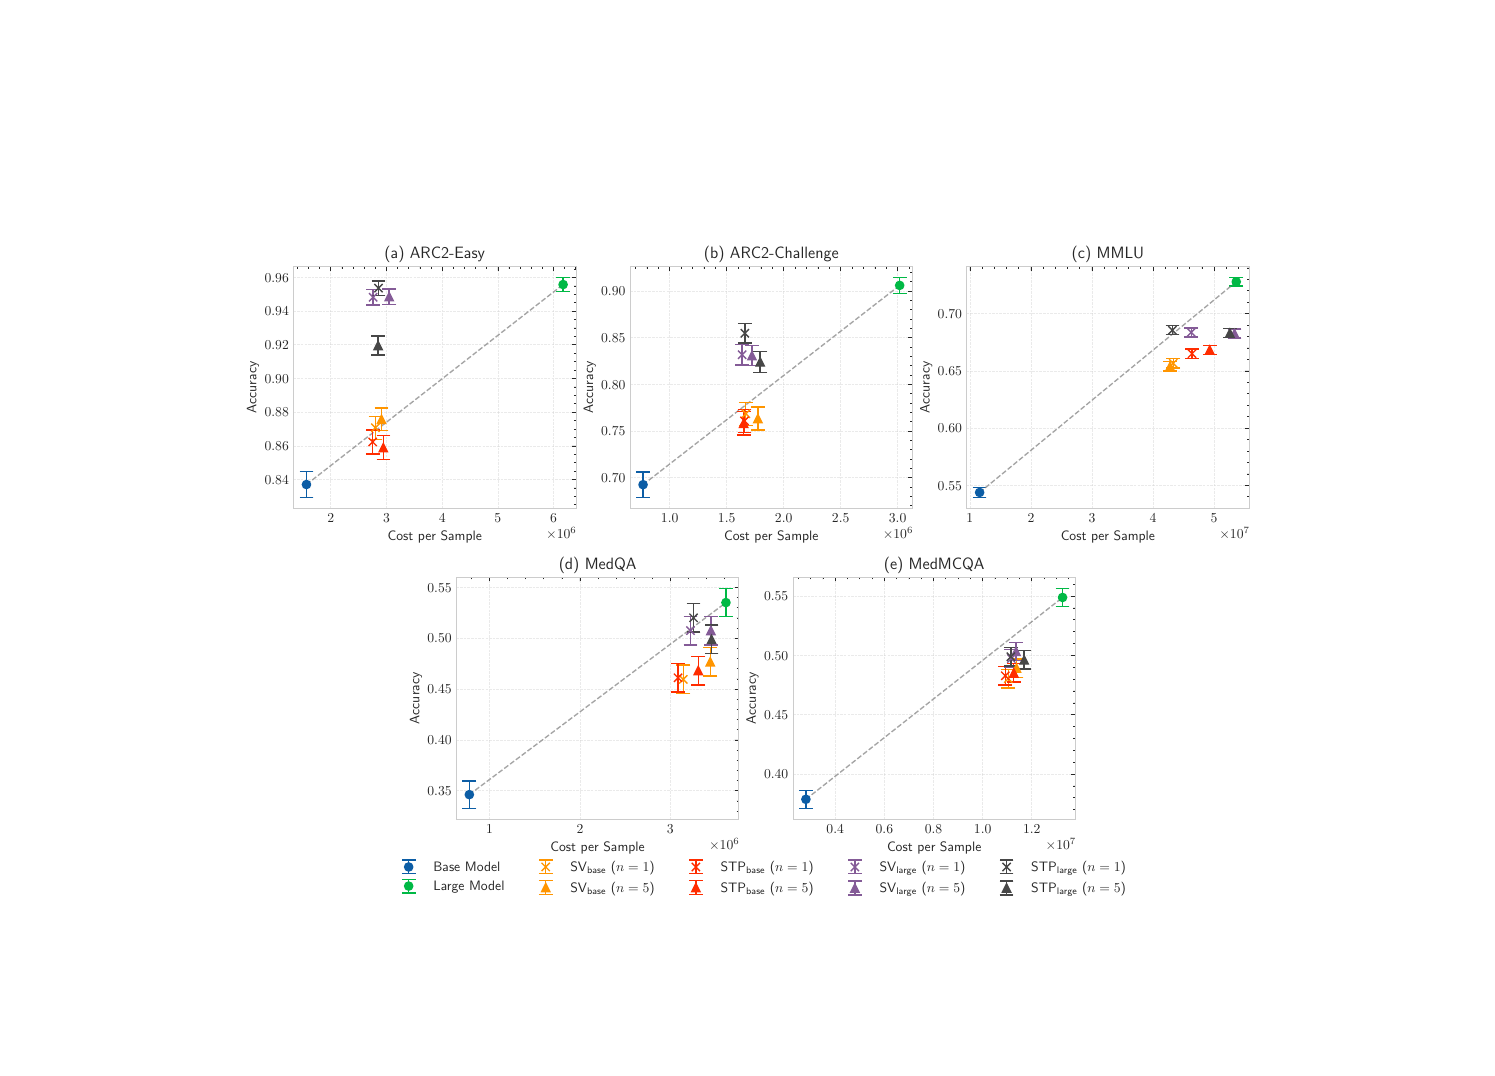
\includegraphics[width=2.676cm]{figures/img/results_gallery/tile_14.png}}};
\draw[black!35,line width=0.35pt] (5.562,-16.084) rectangle (8.238,-18.010);
\node[anchor=north west,text=ACMDarkBlue,font=\tiny\bfseries,inner sep=0] at (5.592,-18.040) {\href{https://arxiv.org/abs/2506.11887}{\adjustbox{max width=2.616cm}{Fanconi and van der Schaar 2025}}};
\node[anchor=north west,text=black!60,font=\tiny,inner sep=0] at (5.592,-18.245) {\href{https://arxiv.org/abs/2506.11887}{Fig. 3, p.~8}};
\node[anchor=north west,inner sep=0] at (8.308,-16.084) {\href{https://arxiv.org/abs/2402.15610}{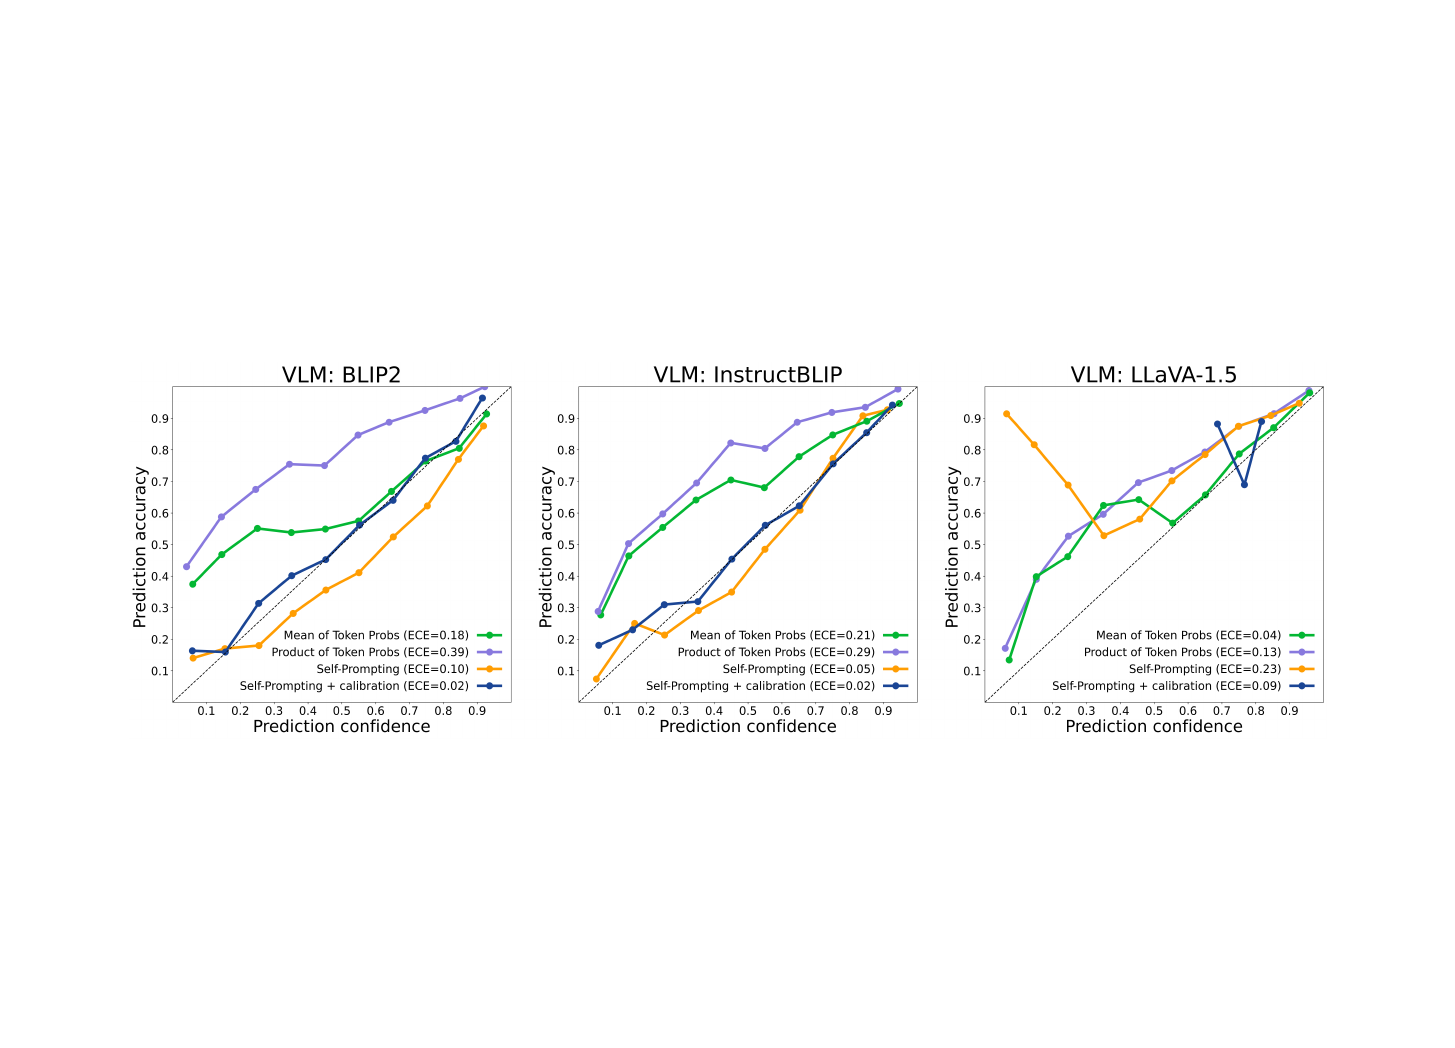
\includegraphics[width=2.676cm]{figures/img/results_gallery/tile_15.png}}};
\draw[black!35,line width=0.35pt] (8.308,-16.084) rectangle (10.984,-18.010);
\node[anchor=north west,text=ACMDarkBlue,font=\tiny\bfseries,inner sep=0] at (8.338,-18.040) {\href{https://arxiv.org/abs/2402.15610}{\adjustbox{max width=2.616cm}{Srinivasan et al. 2024}}};
\node[anchor=north west,text=black!60,font=\tiny,inner sep=0] at (8.338,-18.245) {\href{https://arxiv.org/abs/2402.15610}{Fig. 3, p.~5}};
\end{tikzpicture}}
\caption{\textbf{What calibration looks like in results, by stage.} Each panel shows a whole figure of the cited paper, reproduced under its CC BY licence; its label links to the paper. The selection rule and each panel's figure, page and licence are in Table~\ref{tab:panel_provenance}.}
\Description{A labelled grid of images, each a hyperlink annotated with its system name and source figure number.}
\label{fig:results_gallery}
\end{figure*}

